\chapter{Dapatan Kajian}
\section{Pengenalan}

Bab ini menguraikan secara mendalam hasil penelitian yang menjawab pertanyaan-pertanyaan terkait efektivitas pembelajaran pengenalan huruf menggunakan aplikasi berbasis Augmented Reality (AR) untuk siswa prasekolah. Fokus utama penelitian ini adalah mengidentifikasi kebutuhan teknis dan pedagogis dalam pengembangan aplikasi AR Alphabets, merancang dan membangun aplikasi tersebut, serta mengevaluasi tingkat kegunaan dan penerimaan aplikasi ini di kalangan siswa dan guru sebagai alat pendukung pembelajaran literasi awal. Hasil penelitian ini memberikan wawasan berharga tentang potensi teknologi AR dalam meningkatkan pengalaman belajar anak-anak prasekolah, khususnya dalam pengenalan huruf.

Lebih lanjut, bab ini menjelaskan metodologi yang digunakan dalam penelitian, termasuk proses pengumpulan data, analisis, dan interpretasi hasil. Temuan-temuan yang dipaparkan mencakup aspek-aspek seperti tingkat keterlibatan siswa, peningkatan pemahaman huruf, serta tanggapan guru terhadap penggunaan aplikasi AR dalam pengajaran. Selain itu, bab ini juga membahas tantangan-tantangan yang dihadapi selama implementasi aplikasi dan memberikan rekomendasi untuk pengembangan lebih lanjut. Dengan demikian, bab ini menyajikan gambaran komprehensif tentang potensi dan dampak penggunaan teknologi AR dalam pembelajaran literasi awal di tingkat prasekolah.


\hspace{1cm}{}Hasil dapatan kajian ini diharapkan dapat memberikan pandangan mendalam tentang potensi penggunaan teknologi AR dalam pembelajaran literasi awal di peringkat prasekolah. Analisis terperinci terhadap keperluan teknikal dan pedagogi akan membantu dalam pengoptimuman aplikasi AR Alphabets, manakala penilaian kebolehgunaan dan penerimaan aplikasi oleh pengguna sasaran akan memberikan maklumat berharga untuk penambahbaikan dan pengembangan aplikasi ini pada masa hadapan. Dapatan kajian ini juga berpotensi untuk menyumbang kepada perkembangan kaedah pengajaran dan pembelajaran yang lebih inovatif dan berkesan dalam pendidikan awal kanak-kanak.\\


\begin{table}[h]
\centering
\caption{Ringkasan Ujian, Kaedah dan Lampiran Berkaitan}
\label{jadual:ringkasan_ujian}
\begin{tabular}{>{\centering\arraybackslash}p{6cm}cc}
\toprule
\textbf{Nama Ujian} & \textbf{Kaedah Ujian} & \textbf{Lampiran} \\
 Analisis Keperluan & Borang Soal Selidik &Lampiran A \\ \midrule
Analisis Keperluan & Temu bual Pakar & Lampiran B\\ 
Ujian Alfa (System Usability Scale) & Borang  Ujian Fungsional& Lampiran C \\ 
Ujian Beta (Kebolehgunaan / Penerimaan Pengguna) & Borang Soal Selidik SUS & Lampiran D \\ 
Ujian Pre / Post & Soalan Ujian & Lampiran F \\ 
Kebolehgunaan (Penerimaan Pengguna) & Temu bual Murid / Guru & Lampiran G \\ \bottomrule
\end{tabular}
\end{table}
\clearpage


\section{\textbf{DAPATAN   SATU(1)-Fasa 1-\textit{Dapatan Soal Selidik Analisa Keperluan  berkaitan keperluan penggunaan aplikasi AR dalam pembelajaran huruf}}

\subsection{Demografi Responden Fasa Analisis Keperluan}


Seramai 50 orang pelajar Program Ijazah Sarjana Muda Perguruan (PISMP) dari Zon Utara telah terlibat sebagai responden dalam kajian ini. Dapatan demografi responden meliputi aspek jantina, kerjaya, kelulusan akademik, lokasi pengajian, tahap kemahiran penggunaan ICT, dan jenis alatan teknologi yang dimiliki. Ringkasan profil responden ditunjukkan dalam Jadual~\ref{jadual:demografiResponden}.

\begin{table}[H]
\centering
\caption{Demografi Responden Fasa Analisis Keperluan}
\label{jadual:demografiResponden}
\begin{tabular}{|p{6cm}|p{6cm}|}
\hline
\textbf{Aspek} & \textbf{Peratusan / Bilangan (N)} \\
\hline
Jantina & Lelaki: 40\% (N=20) \newline Perempuan: 60\% (N=30) \\
\hline
Kerjaya & Pelajar sepenuh masa: 100\% (N=50) \\
\hline
Tahap Kelulusan Akademik & Diploma: 60\% (N=30) \newline Ijazah: 30\% (N=15) \newline Sarjana: 10\% (N=5) \\
\hline
Zon Tempat Belajar & Bangsar: (N=10) \newline Pudu: (N=10) \newline Keramat: (N=10) \newline Lain-lain Zon: (N=20) \\
\hline
Tahap Kemahiran Penggunaan ICT & Sederhana Mahir: 56\% (N=28) \newline Sangat Mahir: 44\% (N=22) \\
\hline
\end{tabular}
\end{table}

Daripada jumlah keseluruhan 50 responden, majoriti adalah perempuan (60\%) manakala selebihnya adalah lelaki (40\%). Semua responden merupakan pelajar sepenuh masa dalam program PISMP. Dari segi kelulusan akademik, kebanyakan responden memiliki kelulusan diploma, diikuti ijazah dan sarjana. Tahap kemahiran penggunaan ICT menunjukkan bahawa sebahagian besar responden berada pada tahap sederhana mahir dan sangat mahir, menunjukkan kesediaan mereka untuk menggunakan teknologi dalam pembelajaran.
\subsection{Dapatan Mengikut Konstruk: Objektif Aplikasi}

Konstruk pertama dalam soal selidik merujuk kepada persepsi responden terhadap objektif pembangunan aplikasi \textit{AR Alphabets Prasekolah}. Item-item dalam konstruk ini bertujuan untuk menilai sejauh mana responden bersetuju bahawa aplikasi ini dapat membantu dalam pencapaian objektif pembelajaran huruf di peringkat prasekolah.

Analisis deskriptif menggunakan min dan peratusan telah dijalankan. Jadual~\ref{jadual:objektifAplikasi} menunjukkan skor min bagi setiap item dalam konstruk ini.

\begin{table}[H]
\centering
\caption{Skor Min Bagi Konstruk Objektif Aplikasi}
\label{jadual:objektifAplikasi}
\begin{tabular}{|c|p{9cm}|c|}
\hline
\textbf{Bil} & \textbf{Item} & \textbf{Min} \\
\hline
1 & Aplikasi ini dapat membantu murid mengenal huruf dengan lebih interaktif. & 4.52 \\
\hline
2 & Objektif pembelajaran huruf dapat dicapai dengan bantuan teknologi AR. & 4.36 \\
\hline
3 & Aplikasi ini dapat meningkatkan minat murid terhadap pembelajaran huruf. & 4.48 \\
\hline
4 & Aplikasi ini sesuai digunakan dalam sesi pengajaran dan pembelajaran formal. & 4.22 \\
\hline
5 & Aplikasi ini boleh menyokong objektif kurikulum prasekolah. & 4.40 \\
\hline
\textbf{Purata Min} & & \textbf{4.40} \\
\hline
\end{tabular}
\end{table}

Berdasarkan Jadual~\ref{jadual:objektifAplikasi}, semua item dalam konstruk ini mencatatkan skor min melebihi 4.00, menunjukkan tahap persetujuan yang tinggi dalam kalangan responden. Item tertinggi ialah “Aplikasi ini dapat membantu murid mengenal huruf dengan lebih interaktif” (min = 4.52), manakala item terendah masih berada dalam julat tinggi iaitu “Aplikasi ini sesuai digunakan dalam sesi pengajaran dan pembelajaran formal” (min = 4.22).

Secara keseluruhan, dapatan ini menunjukkan bahawa responden bersetuju bahawa objektif pembelajaran huruf dapat dicapai dengan lebih berkesan melalui penggunaan aplikasi berasaskan teknologi AR.
\subsection{Dapatan Mengikut Konstruk: Isi Kandungan Aplikasi}

Konstruk kedua dalam soal selidik merujuk kepada persepsi responden terhadap isi kandungan yang dicadangkan dalam aplikasi \textit{AR Alphabets Prasekolah}. Item-item dalam konstruk ini bertujuan untuk menilai kesesuaian, keberkesanan, dan kebolehlaksanaan kandungan pembelajaran huruf yang disampaikan melalui aplikasi.

Jadual~\ref{jadual:isiKandungan} menunjukkan skor min bagi setiap item dalam konstruk ini.

\begin{table}[H]
\centering
\caption{Skor Min Bagi Konstruk Isi Kandungan Aplikasi}
\label{jadual:isiKandungan}
\begin{tabular}{|c|p{9cm}|c|}
\hline
\textbf{Bil} & \textbf{Item} & \textbf{Min} \\
\hline
1 & Kandungan aplikasi merangkumi semua huruf abjad A hingga Z. & 4.44 \\
\hline
2 & Setiap huruf disertakan dengan contoh perkataan dan visual. & 4.36 \\
\hline
3 & Kandungan aplikasi sesuai dengan tahap perkembangan murid prasekolah. & 4.48 \\
\hline
4 & Aplikasi menyediakan aktiviti interaktif untuk setiap huruf. & 4.30 \\
\hline
5 & Kandungan aplikasi selaras dengan kurikulum prasekolah semasa. & 4.42 \\
\hline
\textbf{Purata Min} & & \textbf{4.40} \\
\hline
\end{tabular}
\end{table}

Dapatan menunjukkan bahawa semua item dalam konstruk ini memperoleh skor min melebihi 4.00, yang menunjukkan tahap persetujuan yang tinggi. Item tertinggi ialah “Kandungan aplikasi sesuai dengan tahap perkembangan murid prasekolah” (min = 4.48), manakala item terendah ialah “Aplikasi menyediakan aktiviti interaktif untuk setiap huruf” (min = 4.30), namun masih dalam julat tinggi.

Secara keseluruhan, responden bersetuju bahawa isi kandungan aplikasi adalah sesuai, lengkap dan menyokong pembelajaran huruf secara berkesan di peringkat prasekolah.
\subsection{Dapatan Mengikut Konstruk: Jenis Aplikasi}

Konstruk ini menilai persepsi responden terhadap jenis aplikasi yang sesuai digunakan dalam pembelajaran huruf menggunakan teknologi AR. Ia merangkumi aspek interaktiviti, fleksibiliti, dan kesesuaian platform.

\begin{table}[H]
\centering
\caption{Skor Min Bagi Konstruk Jenis Aplikasi}
\label{jadual:jenisAplikasi}
\begin{tabular}{|c|p{9cm}|c|}
\hline
\textbf{Bil} & \textbf{Item} & \textbf{Min} \\
\hline
1 & Aplikasi perlu boleh digunakan pada pelbagai peranti (telefon, tablet, komputer). & 4.46 \\
\hline
2 & Aplikasi perlu boleh digunakan secara dalam talian dan luar talian. & 4.38 \\
\hline
3 & Aplikasi perlu mesra pengguna dan mudah dikendalikan oleh murid. & 4.50 \\
\hline
4 & Aplikasi perlu mempunyai elemen gamifikasi untuk menarik minat murid. & 4.42 \\
\hline
\textbf{Purata Min} & & \textbf{4.44} \\
\hline
\end{tabular}
\end{table}

Dapatan menunjukkan bahawa responden sangat bersetuju bahawa aplikasi perlu fleksibel, mesra pengguna dan menyokong pelbagai peranti. Item tertinggi ialah “Aplikasi perlu mesra pengguna dan mudah dikendalikan oleh murid” (min = 4.50).
\subsection{Dapatan Mengikut Konstruk: Perkakasan}

Konstruk ini menilai jenis perkakasan yang sesuai digunakan untuk menyokong penggunaan aplikasi AR dalam pembelajaran huruf.

\begin{table}[H]
\centering
\caption{Skor Min Bagi Konstruk Perkakasan}
\label{jadual:perkakasan}
\begin{tabular}{|c|p{9cm}|c|}
\hline
\textbf{Bil} & \textbf{Item} & \textbf{Min} \\
\hline
1 & Telefon pintar adalah peranti utama yang sesuai digunakan. & 4.48 \\
\hline
2 & Tablet memberikan paparan yang lebih besar dan sesuai untuk murid. & 4.40 \\
\hline
3 & Komputer riba boleh digunakan oleh guru untuk tujuan pengajaran. & 4.36 \\
\hline
4 & Aplikasi perlu menyokong penggunaan kamera untuk fungsi AR. & 4.52 \\
\hline
\textbf{Purata Min} & & \textbf{4.44} \\
\hline
\end{tabular}
\end{table}

Responden menunjukkan persetujuan tinggi terhadap keperluan perkakasan asas seperti telefon pintar, tablet dan komputer riba. Item tertinggi ialah “Aplikasi perlu menyokong penggunaan kamera untuk fungsi AR” (min = 4.52).
\subsection{Dapatan Mengikut Konstruk: Strategi Pengajaran}

Konstruk ini menilai strategi pengajaran yang sesuai digunakan bersama aplikasi AR dalam pembelajaran huruf.

\begin{table}[H]
\centering
\caption{Skor Min Bagi Konstruk Strategi Pengajaran}
\label{jadual:strategiPengajaran}
\begin{tabular}{|c|p{9cm}|c|}
\hline
\textbf{Bil} & \textbf{Item} & \textbf{Min} \\
\hline
1 & Aplikasi boleh digunakan dalam aktiviti pembelajaran berpusatkan murid. & 4.46 \\
\hline
2 & Aplikasi sesuai digunakan dalam aktiviti kumpulan kecil. & 4.34 \\
\hline
3 & Aplikasi boleh digunakan dalam aktiviti pengayaan dan pemulihan. & 4.40 \\
\hline
\textbf{Purata Min} & & \textbf{4.40} \\
\hline
\end{tabular}
\end{table}

Dapatan menunjukkan bahawa responden bersetuju aplikasi ini sesuai digunakan dalam pelbagai strategi pengajaran, termasuk aktiviti berpusatkan murid dan kumpulan kecil.
\subsection{Dapatan Mengikut Konstruk: Bentuk Penilaian}

Konstruk ini menilai bentuk penilaian yang sesuai dilaksanakan melalui aplikasi AR dalam pembelajaran huruf.

\begin{table}[H]
\centering
\caption{Skor Min Bagi Konstruk Bentuk Penilaian}
\label{jadual:bentukPenilaian}
\begin{tabular}{|c|p{9cm}|c|}
\hline
\textbf{Bil} & \textbf{Item} & \textbf{Min} \\
\hline
1 & Aplikasi boleh menyediakan kuiz interaktif untuk menilai pemahaman murid. & 4.50 \\
\hline
2 & Penilaian boleh dijalankan secara automatik melalui aplikasi. & 4.42 \\
\hline
3 & Aplikasi boleh menyimpan rekod pencapaian murid. & 4.38 \\
\hline
4 & Penilaian melalui aplikasi boleh membantu guru membuat intervensi. & 4.46 \\
\hline
\textbf{Purata Min} & & \textbf{4.44} \\
\hline
\end{tabular}
\end{table}

Responden menunjukkan tahap persetujuan yang tinggi terhadap bentuk penilaian digital yang disediakan oleh aplikasi. Item tertinggi ialah “Aplikasi boleh menyediakan kuiz interaktif untuk menilai pemahaman murid” (min = 4.50).
\section{Rumusan Fasa Analisis Keperluan}

Fasa analisis keperluan merupakan asas penting dalam proses pembangunan aplikasi \textit{AR Alphabets Prasekolah}. Dapatan daripada soal selidik yang melibatkan 50 orang pelajar PISMP Zon Utara menunjukkan tahap persetujuan yang tinggi terhadap keperluan membangunkan aplikasi pembelajaran huruf berasaskan teknologi realiti terimbuh (AR). Semua konstruk yang dikaji—merangkumi objektif aplikasi, isi kandungan, jenis aplikasi, perkakasan, strategi pengajaran, dan bentuk penilaian—mencatatkan skor min melebihi 4.00, yang menunjukkan tahap persetujuan yang tinggi dalam kalangan responden.

Selain itu, dapatan temu bual bersama empat orang pakar turut menyokong keperluan pembangunan aplikasi ini. Tujuh konstruk utama telah dikenalpasti melalui analisis tematik, iaitu objektif aplikasi, isi kandungan, jenis aplikasi, perkakasan, strategi pengajaran dan pembelajaran, bentuk penilaian, serta peluang pelaksanaan. Pandangan pakar mengesahkan bahawa aplikasi ini berpotensi untuk menyokong pengajaran huruf secara lebih interaktif, fleksibel dan selaras dengan perkembangan teknologi pendidikan semasa.

Secara keseluruhannya, dapatan fasa ini memberikan justifikasi yang kukuh terhadap keperluan membangunkan aplikasi \textit{AR Alphabets Prasekolah}. Maklumat yang diperoleh menjadi asas penting dalam mereka bentuk kandungan, fungsi dan strategi pelaksanaan aplikasi yang akan dibangunkan dalam fasa seterusnya.
\section{P

\section{\textbf{Dapatan Dua(2)}-Fasa 1-\textit{Dapatan Temu Bual Pakar berkaitan keperluan penggunaan aplikasi AR dalam pembelajaran huruf}}


Fasa analisis keperluan dalam pembangunan aplikasi AR Alphabets merangkumi pelbagai aspek yang perlu dipertimbangkan dengan teliti. Selain mengenal pasti keperluan pengguna dan memastikan kesesuaian dengan tahap perkembangan literasi awal kanak-kanak prasekolah, fasa ini juga melibatkan penelitian terhadap elemen-elemen teknikal dan pedagogi. Reka bentuk aplikasi perlu dirancang dengan teliti untuk memastikan antara muka yang mesra pengguna dan menarik minat kanak-kanak. Pemilihan perkakasan yang sesuai dan platform pembangunan yang tepat adalah penting untuk memastikan aplikasi dapat berfungsi dengan lancar dan mudah diakses oleh pengguna sasaran.\\

\hspace{1cm}Kandungan pengajaran dan strategi PdP yang diintegrasikan dalam aplikasi AR Alphabets perlu disesuaikan dengan keperluan pembelajaran kanak-kanak prasekolah. Ini termasuk memastikan kandungan yang interaktif, menarik, dan sesuai dengan tahap kognitif mereka. Bentuk penilaian yang dimasukkan dalam aplikasi juga perlu direka dengan teliti untuk membolehkan pemantauan kemajuan pembelajaran kanak-kanak secara berkesan. Akhir sekali, potensi pelaksanaan aplikasi AR dalam konteks pendidikan awal kanak-kanak perlu dinilai dari segi keberkesanan, kesesuaian, dan kemampuan untuk meningkatkan pengalaman pembelajaran. Semua aspek ini perlu dianalisis dan diintegrasikan dengan baik untuk memastikan aplikasi AR Alphabets dapat memenuhi objektif pembelajaran dan memberi impak positif terhadap perkembangan literasi awal kanak-kanak prasekolah.\\


\hspace{1cm}Hasil daripada fasa analisis keperluan ini akan memberi impak yang signifikan terhadap keseluruhan proses pembangunan aplikasi AR Alphabets. Maklumat yang diperoleh daripada pakar-pakar dalam bidang pendidikan awal kanak-kanak dan teknologi pendidikan akan membantu memastikan aplikasi yang dibangunkan bukan sahaja memenuhi keperluan teknikal, tetapi juga bersesuaian dengan keperluan pedagogi dan perkembangan kognitif kanak-kanak prasekolah. Pendekatan ini akan membantu menghasilkan aplikasi AR yang lebih efektif dan bermakna dalam menyokong pembelajaran literasi awal

\subsection{Pandangan Pakar terhadap Keperluan Reka Bentuk Model Aplikasi \textit{AR Alphabets}}

\begin{quote}\begin{center}\textbf{.......................} \textit{"Menurut saya, model aplikasi \textit{AR Alphabets} sangat diperlukan dalam kelas. Ini sejalan dengan era pendidikan abad ke-21 yang menuntut penggunaan media interaktif sebagai platform pembelajaran yang efektif."} (\textbf{P1})\end{center}\end{quote}\\
\begin{quote}
\begin{center}
\textbf{.......................} \textit{"Ya… perlu… kerana perubahan ketara dalam sistem pendidikan negara dan di peringkat global memerlukan kaedah P\&P diajar dan diamalkan dengan cara dinamik; tidak hanya bertumpu kepada pembelajaran dalam kelas, tetapi proses P\&P boleh berlaku di mana sahaja. Jadi, \textit{mobile learning} semakin signifikan."} (\textbf{P2})\end{center}\\
\end{quote}\\

Pembangunan aplikasi AR Alphabets merupakan langkah penting dalam evolusi pendidikan kontemporari. Ia bukan sahaja memenuhi keperluan pedagogi abad ke-21, tetapi juga menyediakan platform pembelajaran yang interaktif dan menarik. Aplikasi ini menggabungkan teknologi realiti terimbuh (AR) dengan pembelajaran abjad, mencipta pengalaman pendidikan yang imersif dan dinamik. Pendekatan ini membolehkan pelajar berinteraksi dengan huruf-huruf dalam persekitaran 3D, meningkatkan pemahaman dan pengekalan maklumat melalui penglibatan visual dan kinestetik.

Selain itu, AR Alphabets menyokong konsep pembelajaran fleksibel yang semakin penting dalam era digital ini. Ia membolehkan pelajar mengakses bahan pembelajaran di mana-mana dan pada bila-bila masa, menggalakkan pembelajaran kendiri dan menyesuaikan diri dengan pelbagai gaya pembelajaran. Penggunaan teknologi AR dalam pendidikan awal kanak-kanak juga membantu memupuk kemahiran literasi digital yang penting untuk kejayaan masa depan. Oleh itu, pembangunan aplikasi seperti AR Alphabets bukan sahaja selaras dengan tuntutan pendidikan moden, tetapi juga menyediakan asas yang kukuh untuk pembelajaran sepanjang hayat dalam dunia yang semakin didorong oleh teknologi.

\subsection{Pandangan Pakar terhadap Jenis Perkakasan Teknologi Mudah Alih}

\begin{quote}\begin{center}\textbf{.......................} \textit{"Menurut saya, jenis perkakasan utama yang paling sesuai untuk kursus ini adalah seperti iPad, smartphone, dan juga tablet."} (\textbf{P1})\end{center}\end{quote}\\
\begin{quote}
\begin{center}
\textbf{.......................} \textit{"Telefon pintar dan tablet. Lihat juga pada komputer riba... agak sesuai juga kerana ia merupakan komputer mudah alih."} (\textbf{P2})\end{center}
\end{quote}\\

Kedua-dua responden menyatakan bahawa peranti seperti telefon pintar dan tablet merupakan perkakasan yang paling sesuai. Mereka juga membincangkan tentang komputer riba dan netbook sebagai alternatif dalam pelaksanaan aplikasi pembelajaran mudah alih.Peranti mudah alih seperti telefon pintar dan tablet dianggap sebagai perkakasan yang paling sesuai untuk aplikasi pembelajaran mudah alih menurut kedua-dua responden. Ciri-ciri seperti saiz yang kompak, mudah dibawa, dan keupayaan untuk mengakses internet di mana-mana sahaja menjadikan peranti ini pilihan utama. Telefon pintar dan tablet juga menawarkan pelbagai fungsi seperti kamera, mikrofon, dan skrin sentuh yang boleh dimanfaatkan dalam pelbagai aktiviti pembelajaran interaktif.

Selain itu, responden turut membincangkan komputer riba dan netbook sebagai alternatif yang berpotensi untuk pelaksanaan aplikasi pembelajaran mudah alih. Walaupun kurang mudah alih berbanding telefon pintar dan tablet, peranti ini menawarkan kelebihan seperti skrin yang lebih besar dan papan kekunci fizikal yang boleh memudahkan penulisan dan penggunaan aplikasi yang lebih kompleks. Pilihan antara peranti-peranti ini bergantung kepada keperluan spesifik program pembelajaran, keutamaan pengguna, dan konteks penggunaan.

\subsection{{Pandangan Pakar terhadap Pelbagai Jenis Aplikasi / Platform Teknologi Mudah Alih}}

\begin{quote}\begin{center}\textbf{.......................} \textit{"Bagi saya, aplikasi Unity adalah pilihan yang sangat penting. Ini kerana Unity digunakan untuk membangunkan aplikasi Augmented Reality, yang menjadikan pembelajaran lebih berkesan."} (\textbf{P1})\end{center}\end{quote}\\
\begin{quote}
\begin{center}\textbf{.......................} \textit{"Vuforia diperlukan untuk memadankan sistem marker, dan pembelajaran akan menjadi lebih berkesan."} (\textbf{P2})\end{center}\end{quote}\\
Pakar menegaskan bahawa pemilihan platform pembangunan yang tepat seperti Unity dan Vuforia adalah penting bagi menjamin keberkesanan dan kefungsian aplikasi \textit{AR Alphabets}.


\subsection{Pandangan Pakar terhadap Aktiviti Pengajaran dan Pembelajaran yang Sesuai}


\begin{quote}
\begin{center}
\textbf{.......................} \textit{"Pada saya, aktiviti mengenal huruf semestinya perlu dimasukkan."} (\textbf{P1})
\end{center}
\end{quote}\\

\begin{quote}
\begin{center}
\textbf{.......................} \textit{"Kuiz dan permainan."} (\textbf{P2})
\end{center}
\end{quote}\\

Kedua-dua pakar menyatakan bahawa elemen aktiviti adalah tunjang utama dalam aplikasi pendidikan digital. Aktiviti seperti mengenal huruf, kuiz dan permainan mampu meningkatkan tumpuan dan motivasi murid semasa proses PdP.

\subsection{Pandangan Pakar terhadap Strategi Pengajaran yang Sesuai}


\begin{quote}
\begin{center}
\textbf{.......................} \textit{"Strategi yang sesuai adalah strategi pengajaran langsung dan juga strategi P\&P menggunakan media interaktif."} (\textbf{P1})
\end{center}
\end{quote}\\

\begin{quote}
\begin{center}
\textbf{.......................} \textit{"Penggunaan media interaktif."} (\textbf{P2})
\end{center}
\end{quote}\\

Pakar bersetuju bahawa strategi yang berasaskan interaktiviti dan pengajaran langsung amat sesuai. Strategi ini juga seiring dengan pendekatan teori Konstruktivis yang menyokong pembelajaran aktif dan pengalaman kendiri.

\subsection{Pandangan Pakar terhadap Bentuk Penilaian yang Sesuai}


\begin{quote}
\begin{center}
\textbf{.......................} \textit{"Penghasilan permainan, kuiz yang mempunyai sistem mata."} (\textbf{P1})
\end{center}
\end{quote}\\

\begin{quote}
\begin{center}
\textbf{.......................} \textit{"Permainan, kuiz yang menguji murid."} (\textbf{P2})
\end{center}
\end{quote}\\

Kedua-dua pakar berpendapat bahawa bentuk penilaian seperti kuiz, permainan berasaskan skor, dan penilaian kendiri secara interaktif mampu memberi maklum balas terus kepada murid serta mendorong minat belajar.

\subsection{Pandangan Pakar terhadap Peluang Pelaksanaan P\&P Berdasarkan Aplikasi }

\begin{quote}
\begin{center}
\textbf{.......................} \textit{"Sesuai dilaksanakan. Murid akan menjadi lebih yakin bila menggunakan \textit{device} dan model P\&P secara serentak untuk proses pengajaran dan pembelajaran."} (\textbf{P1})
\end{center}
\end{quote}\\

\begin{quote}
\begin{center}
\textbf{.......................} \textit{"Kerana kaedah \textit{mobile learning} telah semakin berkembang dan diterima oleh masyarakat Malaysia... Pelajar kini lebih terbuka dengan teknologi, dan mereka perlu dipersiapkan untuk generasi seterusnya. Kita tidak boleh hanya tunggu dan lihat; kita perlu jadi sebahagian daripada perkembangan teknologi hari ini."} (\textbf{P2})
\end{center}
\end{quote}\\

Pakar menekankan bahawa pelaksanaan m-Pembelajaran berpotensi tinggi untuk diaplikasikan secara meluas, khususnya dalam kalangan pelajar prasekolah dan institusi latihan perguruan. Pelaksanaan ini dilihat bersesuaian dengan keperluan dan arah pendidikan masa kini.
\clearpage


\subsection{Rumusan Dapatan Kajian Fasa Satu: Analisis Keperluan}

Secara keseluruhannya, dapatan daripada temu bual pakar dalam Fasa Satu menunjukkan bahawa pembinaan aplikasi \textit{AR Alphabets} adalah sangat diperlukan dan signifikan dalam konteks pendidikan prasekolah. Kesemua pakar yang ditemu bual menyatakan persetujuan terhadap aspek-aspek utama dalam reka bentuk dan pembangunan aplikasi ini, termasuk keperluan model pembelajaran yang interaktif, penggunaan teknologi mudah alih yang sesuai, pilihan platform pembangunan seperti Unity dan Vuforia, serta kandungan aktiviti pengajaran dan pembelajaran yang menarik.

Pakar juga bersetuju bahawa strategi pengajaran yang menggunakan media interaktif dan pendekatan konstruktivis amat sesuai untuk menyokong aplikasi ini. Di samping itu, penilaian berasaskan aktiviti seperti kuiz dan permainan dilihat berupaya mengukur keberkesanan pembelajaran secara autentik dan menyeronokkan.

Akhir sekali, para pakar menyatakan bahawa pelaksanaan m-Pembelajaran melalui aplikasi seperti \textit{AR Alphabets} berpotensi untuk dilaksanakan secara menyeluruh dalam sistem pendidikan, selaras dengan perkembangan teknologi digital masa kini dan keperluan pendidikan abad ke-21. Maka, dapatan ini menjadi asas yang kukuh untuk pembangunan seterusnya dalam fasa reka bentuk aplikasi \textit{AR Alphabets}.

\clearpage

\section{{\textbf{Dapatan Tiga (3)-Fasa 2}\textit{-Ujian Alfa (Ujian Fungsional-)}}}
\addcontentsline{toc}{subsection}{Dapatan Ujian Alfa (Ujian Fungsional)}

Ujian Alfa dijalankan oleh pembangun aplikasi untuk menguji semua fungsi utama aplikasi sebelum ia diedarkan kepada pengguna sasaran. Ujian ini memberi fokus kepada fungsi antara muka pengguna, khususnya terhadap setiap butang navigasi dalam modul-modul pembelajaran. Ujian dilakukan secara sistematik dengan menekan butang pada setiap paparan antara muka dan memerhati respons aplikasi secara langsung.

\subsection{{Ujian fungsional bagi butang pada antara muka utama Splash Flash}}
\begin{table}[h]
\centering
\caption{Ujian fungsional bagi butang pada antara muka utama Splash Flash}
\label{jadual-5-1}
\begin{tabular}{lll}
\toprule
\textbf{Item} & \textbf{Keputusan Ujian} & \textbf{Keputusan Sebenar} \\ \midrule
Butang Splash Flash & Navigasi ke List Menu & Berfungsi \\ \bottomrule
\end{tabular}
\end{table}

\begin{figure}[h]
\centering
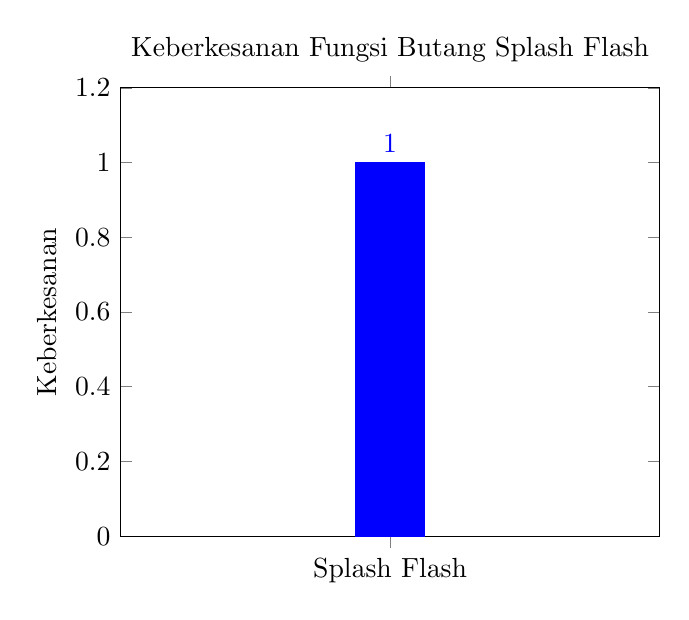
\begin{tikzpicture}
\begin{axis}[
    ybar,
    bar width=25pt,
    enlarge x limits=0.5,
    ymin=0, ymax=1.2,
    ylabel={Keberkesanan},
    symbolic x coords={Splash Flash},
    xtick=data,
    nodes near coords,
    nodes near coords align={vertical},
    title={Keberkesanan Fungsi Butang Splash Flash},
]
\addplot+[fill=blue] coordinates {(Splash Flash,1)};
\end{axis}
\end{tikzpicture}
\caption{Graf Keberkesanan Fungsi Butang Splash Flash}
\end{figure}

\begin{itemize}[h]
  \item 100\% fungsi butang Splash Flash berjaya menavigasi pengguna ke senarai menu.  
  \item Tiada sebarang ralat teknikal dikesan semasa interaksi dengan Splash Flash.  
  \item Keberkesanan fungsi Splash Flash dinilai sempurna (nilai keberkesanan = 1.0).  
  \item Modul utama sedia untuk fasa seterusnya (Ujian Beta) kerana kestabilan fungsi Splash Flash telah disahkan.  
\end{itemize}
\clearpage

\subsection{Ujian fungsional bagi butang antara muka (Modul 1)}
\begin{table}[h]
\centering
\caption{Ujian fungsional bagi butang antara muka (Modul 1)}
\label{jadual-5-2}
\begin{tabular}{|l|l|l|}
\hline
\textbf{Item} & \textbf{Keputusan Ujian} & \textbf{Keputusan Sebenar} \\ \hline
Butang Ke Modul 1 & Navigasi ke Modul 1 & Berfungsi \\ \hline
Butang Ke Modul 2 & Navigasi ke Modul 1 & Berfungsi \\ \hline
Butang Ke Modul 3 & Navigasi ke Modul 1 & Berfungsi \\ \hline
Butang Ke Modul 4 & Navigasi ke Modul 1 & Berfungsi \\ \hline
Butang Ke Modul 5 & Navigasi ke Modul 1 & Berfungsi \\ \hline
Butang Ke Modul 6 & Navigasi ke Modul 1 & Berfungsi \\ \hline
Butang Ke Modul 7 & Navigasi ke Modul 1 & Berfungsi \\ \hline
\end{tabular}
\end{table}

\begin{figure}[h]
\centering
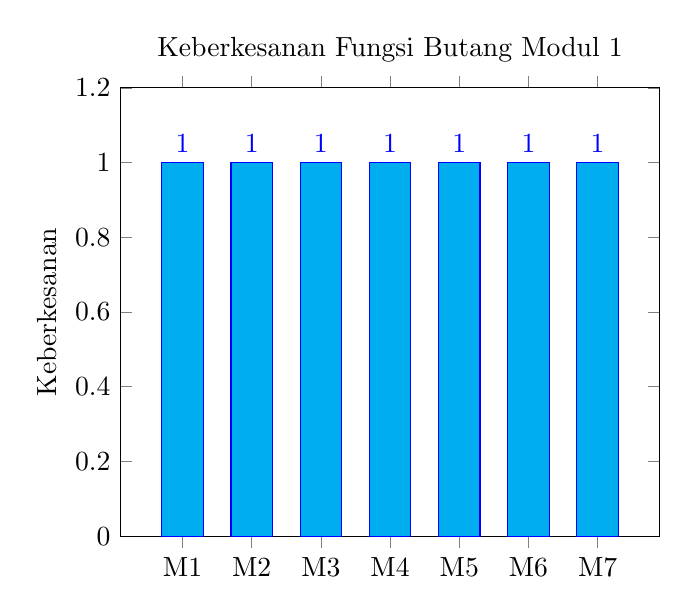
\begin{tikzpicture}
\begin{axis}[
    ybar,
    bar width=15pt,
    enlarge x limits=0.15,
    ymin=0, ymax=1.2,
    ylabel={Keberkesanan},
    symbolic x coords={M1, M2, M3, M4, M5, M6, M7},
    xtick=data,
    nodes near coords,
    nodes near coords align={vertical},
    title={Keberkesanan Fungsi Butang Modul 1},
]
\addplot+[fill=cyan] coordinates {
    (M1,1) (M2,1) (M3,1) (M4,1) (M5,1) (M6,1) (M7,1)
};
\end{axis}
\end{tikzpicture}
\caption{Graf Keberkesanan Fungsi Butang Modul 1}
\label{rajah-5-2}
\end{figure}

\subsubsection{Rumusan Ujian Alfa – Modul 1}

Berdasarkan Jadual~\ref{jadual-5-2}, semua butang navigasi Modul 1–7 berfungsi dengan sempurna. Tiada ralat teknikal dikesan dan setiap interaksi berjaya membawa pengguna ke Modul 1 seperti yang dirancang. Keberkesanan fungsi navigasi modul ini dinilai 100\%, menandakan kestabilan modul untuk fase ujian seterusnya.

\begin{itemize}[h]
  \item Butang Ke Modul 1–7: navigasi tepat ke Modul 1.
  \item Tiada butang yang gagal atau memaparkan ralat.
  \item Kesediaan modul untuk dipertandingkan dalam Ujian Beta disahkan.
\end{itemize}
\clearpage



\subsection{Ujian fungsional antara muka Modul 2}
\begin{table}[h]
\centering
\caption{Ujian fungsional antara muka (Modul 2)}
\begin{tabular}{lll}
\toprule
\textbf{Item} & \textbf{Keputusan Ujian} & \textbf{Keputusan Sebenar} \\ \midrule
Butang Touch Screen Next & Navigasi akan maju ke hadapan & Berfungsi \\ 
Butang Touch Screen Prev & Navigasi kembali & Berfungsi \\ 
Butang Bunyi Haiwan & Navigasi akan memberi isyarat bunyi & Berfungsi \\ \bottomrule
\end{tabular}
\end{table}

\begin{figure}[h]
\centering
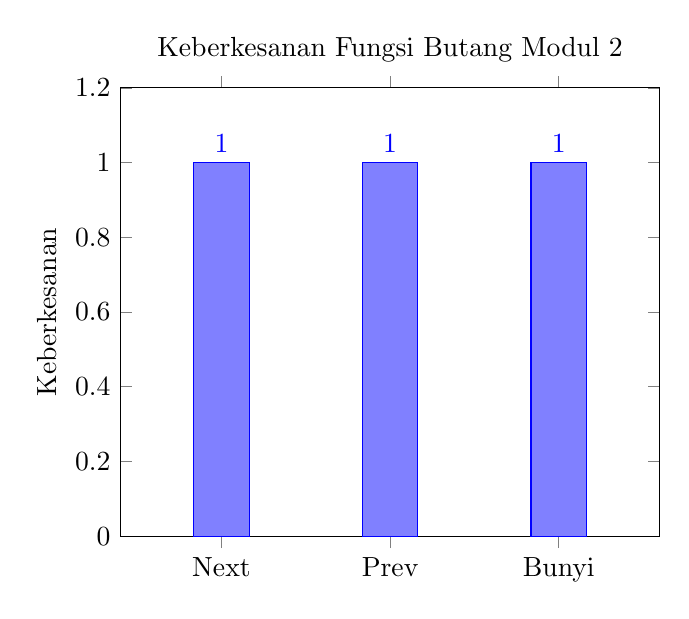
\begin{tikzpicture}
\begin{axis}[
    ybar,
    bar width=20pt,
    enlarge x limits=0.3,
    ymin=0, ymax=1.2,
    ylabel={Keberkesanan},
    symbolic x coords={Next, Prev, Bunyi},
    xtick=data,
    nodes near coords,
    nodes near coords align={vertical},
    title={Keberkesanan Fungsi Butang Modul 2},
]
\addplot+[fill=blue!50] coordinates {
    (Next,1)
    (Prev,1)
    (Bunyi,1)
};
\end{axis}
\end{tikzpicture}
\caption{Graf Keberkesanan Fungsi Butang Modul 2}
\label{rajah-5-3}
\end{figure}
\subsubsection{Rumusan Ujian Alfa – Modul 2}

\begin{itemize}[h]
  \item Butang \textit{Next} dan \textit{Prev} berfungsi dengan tepat memajukan dan mengembalikan skrin.
  \item Butang \textit{Bunyi Haiwan} berjaya mengeluarkan isyarat bunyi seperti yang diharapkan.
  \item Tiada ralat teknikal dikesan dalam semua fungsi Modul 2.
  \item Keberkesanan fungsi Modul 2 dinilai 100\% (nilai keberkesanan = 1.0), menunjukkan modul ini stabil dan sedia untuk Ujian Beta.
\end{itemize}
\clearpage

\subsection{Ujian fungsional antara muka (Modul 3)}
\begin{table}[h]
\centering
\caption{Ujian fungsional antara muka (Modul 3)}
\label{jadual-5-4}
\begin{tabular}{|l|l|l|}
\hline
\textbf{Item} & \textbf{Keputusan Ujian} & \textbf{Keputusan Sebenar} \\ \hline
Butang Touch Screen Next & Navigasi akan maju ke hadapan & Berfungsi \\ \hline
Butang Touch Screen Prev & Navigasi kembali & Berfungsi \\ \hline
Butang Bunyi Haiwan & Navigasi akan memberi isyarat bunyi & Berfungsi \\ \hline
\end{tabular}
\end{table}

\begin{figure}[h]
\centering
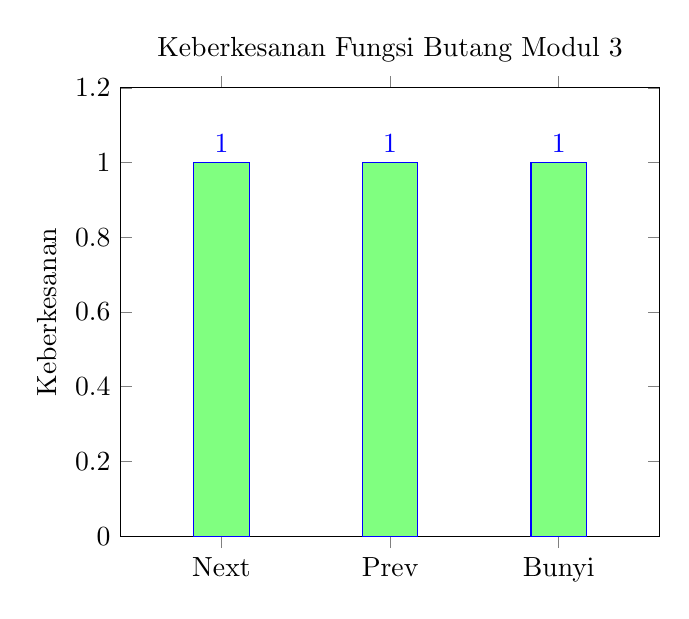
\begin{tikzpicture}
\begin{axis}[
    ybar,
    bar width=20pt,
    enlarge x limits=0.3,
    ymin=0, ymax=1.2,
    ylabel={Keberkesanan},
    symbolic x coords={Next, Prev, Bunyi},
    xtick=data,
    nodes near coords,
    nodes near coords align={vertical},
    title={Keberkesanan Fungsi Butang Modul 3},
]
\addplot+[fill=green!50] coordinates {
    (Next,1)
    (Prev,1)
    (Bunyi,1)
};
\end{axis}
\end{tikzpicture}
\caption{Graf Keberkesanan Fungsi Butang Modul 3}
\label{rajah-5-4}
\end{figure}

\subsubsection{Rumusan Ujian Alfa – Modul 3}

\begin{itemize}[h]
  \item Butang \textit{Touch Screen Next} berfungsi memajukan skrin seperti yang dirancang.
  \item Butang \textit{Touch Screen Prev} berjaya mengembalikan skrin sebelumnya tanpa sebarang ralat.
  \item Butang \textit{Bunyi Haiwan} mengeluarkan isyarat bunyi dengan tepat.
  \item Keberkesanan keseluruhan fungsi Modul 3 adalah 100\%, menandakan modul ini stabil dan sedia untuk fasa Ujian Beta.
\end{itemize}
\clearpage

\subsection{Ujian fungsional antara muka (Modul 4)}
\begin{table}[h]
\centering
\caption{Ujian fungsional antara muka (Modul 4)}
\label{jadual-5-5}
\begin{tabular}{|l|l|l|}
\hline
\textbf{Item} & \textbf{Keputusan Ujian} & \textbf{Keputusan Sebenar} \\ \hline
Butang Touch Screen Next & Navigasi akan maju ke hadapan & Berfungsi \\ \hline
Butang Touch Screen Prev & Navigasi kembali & Berfungsi \\ \hline
Butang Bunyi Haiwan & Navigasi akan memberi isyarat bunyi & Berfungsi \\ \hline
\end{tabular}
\end{table}

\begin{figure}[h]
\centering
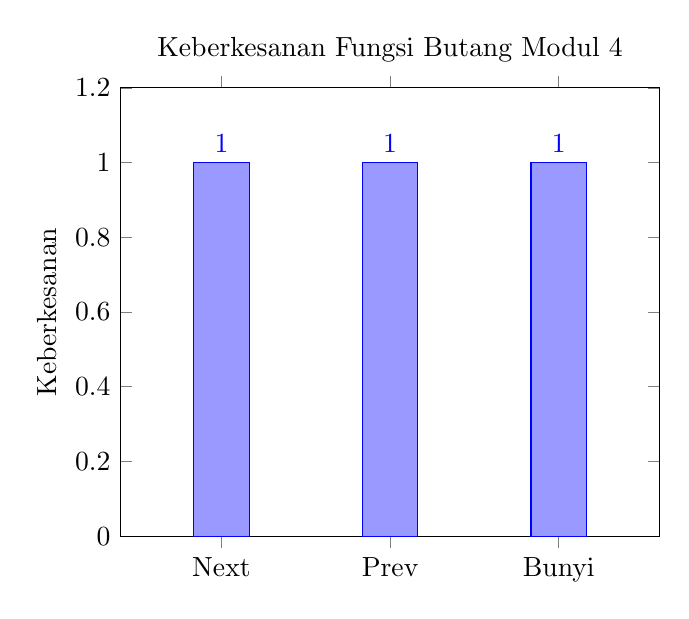
\begin{tikzpicture}
\begin{axis}[
    ybar,
    bar width=20pt,
    enlarge x limits=0.3,
    ymin=0, ymax=1.2,
    ylabel={Keberkesanan},
    symbolic x coords={Next, Prev, Bunyi},
    xtick=data,
    nodes near coords,
    nodes near coords align={vertical},
    title={Keberkesanan Fungsi Butang Modul 4},
]
\addplot+[fill=blue!40] coordinates {
    (Next,1)
    (Prev,1)
    (Bunyi,1)
};
\end{axis}
\end{tikzpicture}
\caption{Graf Keberkesanan Fungsi Butang Modul 4}
\label{rajah-5-5}
\end{figure}
Rumusan Ujian Alfa – Modul 4

\begin{itemize}[h]
  \item Butang \textit{Touch Screen Next} berfungsi memajukan skrin tanpa sebarang ralat.  
  \item Butang \textit{Touch Screen Prev} berjaya mengembalikan skrin seperti yang dirancang.  
  \item Butang \textit{Bunyi Haiwan} mengeluarkan isyarat bunyi dengan tepat.  
  \item Keberkesanan fungsi Modul 4 dinilai sempurna (100\%), menandakan kestabilan modul untuk fasa Ujian Beta.
\end{itemize}
\clearpage

\subsection{Ujian fungsional antara muka (Modul 5)}
\begin{table}[h]
\centering
\caption{Ujian fungsional antara muka (Modul 5)}
\label{jadual-5-6}
\begin{tabular}{lll}
\toprule
\textbf{Item} & \textbf{Keputusan Ujian} & \textbf{Keputusan Sebenar} \\ \midrule
Butang Item Modul & Navigasi dalam antara muka Arahan & Berfungsi \\ 
Butang Kembali & Navigasi kembali & Berfungsi \\ 
Butang Touch Screen Next & Navigasi akan maju ke hadapan & Berfungsi \\ 
Butang Touch Screen Prev & Navigasi kembali & Berfungsi \\ \bottomrule
\end{tabular}
\end{table}

\begin{figure}[h]
\centering
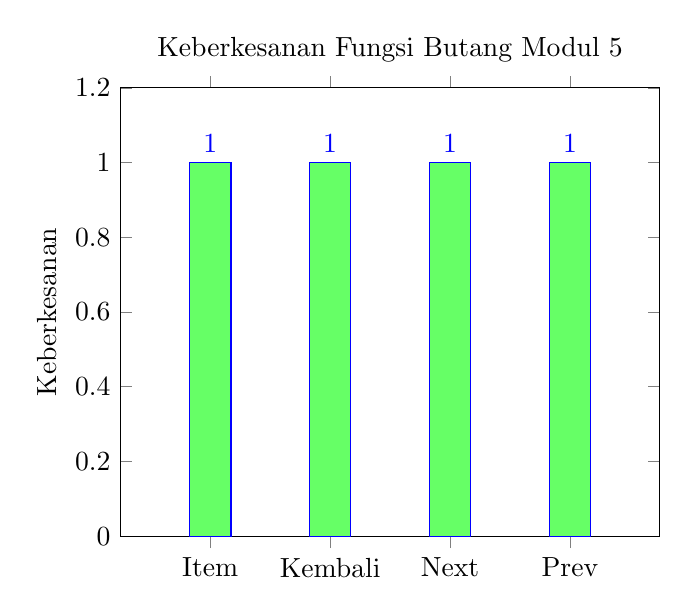
\begin{tikzpicture}
\begin{axis}[
    ybar,
    bar width=15pt,
    enlarge x limits=0.25,
    ymin=0, ymax=1.2,
    ylabel={Keberkesanan},
    symbolic x coords={Item, Kembali, Next, Prev},
    xtick=data,
    nodes near coords,
    nodes near coords align={vertical},
    title={Keberkesanan Fungsi Butang Modul 5},
]
\addplot+[fill=green!60] coordinates {
    (Item,1)
    (Kembali,1)
    (Next,1)
    (Prev,1)
};
\end{axis}
\end{tikzpicture}
\caption{Graf Keberkesanan Fungsi Butang Modul 5}
\label{rajah-5-6}
\end{figure}

 Rumusan Ujian Alfa – Modul 5

\begin{itemize}[h]
  \item Butang \textit{Item Modul} berfungsi dengan tepat, membolehkan navigasi dalam antara muka arahan.  
  \item Butang \textit{Kembali} dan \textit{Prev} mengembalikan pengguna kepada skrin sebelumnya tanpa ralat.  
  \item Butang \textit{Next} memajukan skrin ke modul seterusnya dengan sempurna.  
  \item Keberkesanan keseluruhan fungsi Modul 5 dinilai 100\%, menandakan modul ini stabil dan sedia untuk Ujian Beta.
\end{itemize}
\clearpage

\begin{table}[h]
\centering
\caption{Ujian fungsional antara muka (Modul 6)}
\label{jadual-5-7}
\begin{tabular}{lll}
\toprule
\textbf{Item} & \textbf{Keputusan Ujian} & \textbf{Keputusan Sebenar} \\ \midrule
Butang Item Modul & Navigasi dalam antara muka Arahan & Berfungsi \\ 
Butang Kembali & Navigasi kembali & Berfungsi \\ 
Butang Touch Screen Next & Navigasi akan maju ke hadapan & Berfungsi \\ 
Butang Touch Screen Prev & Navigasi kembali & Berfungsi \\ \bottomrule
\end{tabular}
\end{table}

\begin{figure}[h]
\centering
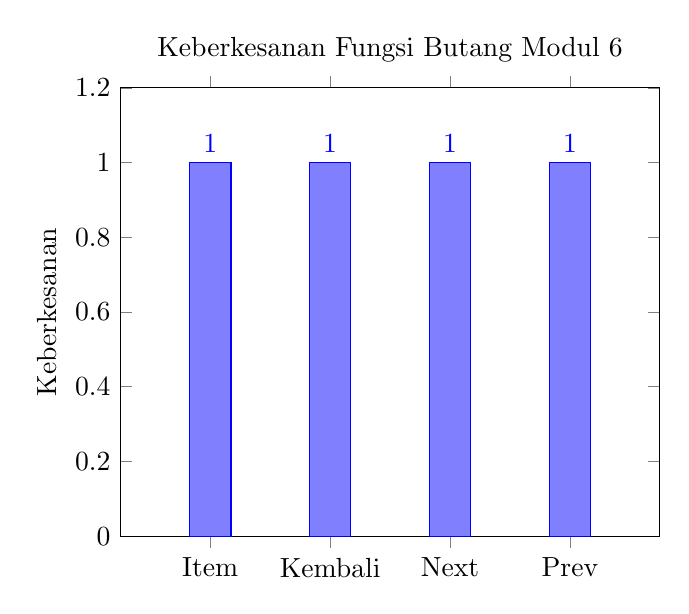
\begin{tikzpicture}
\begin{axis}[
    ybar,
    bar width=15pt,
    enlarge x limits=0.25,
    ymin=0, ymax=1.2,
    ylabel={Keberkesanan},
    symbolic x coords={Item, Kembali, Next, Prev},
    xtick=data,
    nodes near coords,
    nodes near coords align={vertical},
    title={Keberkesanan Fungsi Butang Modul 6},
]
\addplot+[fill=blue!50] coordinates {
    (Item,1)
    (Kembali,1)
    (Next,1)
    (Prev,1)
};
\end{axis}
\end{tikzpicture}
\caption{Graf Keberkesanan Fungsi Butang Modul 6}
\label{rajah-5-7}
\end{figure}

\subsubsection{Rumusan Ujian Alfa – Modul 6}

Berdasarkan Jadual~\ref{jadual-5-7} dan Rajah~\ref{rajah-5-7}:

\begin{itemize}[h]
  \item Butang \textit{Item Modul} berfungsi dengan betul untuk navigasi dalam antara muka arahan.
  \item Butang \textit{Kembali} berjaya membawa pengguna kembali ke skrin sebelumnya tanpa sebarang ralat.
  \item Butang \textit{Touch Screen Next} dan \textit{Prev} memajukan dan mengembalikan skrin seperti yang diharapkan.
  \item Keberkesanan fungsi Modul 6 dinilai 100\%, menandakan kestabilan modul untuk fasa ujian Beta.
\end{itemize}
\clearpage
\begin{table}[H]
\centering
\caption{Ujian fungsional antara muka (Modul 7)}
\label{jadual-5-8}
\begin{tabular}{lll}
\toprule
\textbf{Item} & \textbf{Keputusan Ujian} & \textbf{Keputusan Sebenar} \\ \midrule
Butang Item Modul & Navigasi dalam antara muka Arahan & Berfungsi \\ 
Butang Kembali & Navigasi kembali & Berfungsi \\ 
Butang Touch Screen Next & Navigasi akan maju ke hadapan & Berfungsi \\ 
Butang Touch Screen Prev & Navigasi kembali & Berfungsi \\ 
Butang Audio & Navigasi memberi isyarat audio & Berfungsi \\ 
Butang Image & Navigasi memberi isyarat imej & Berfungsi \\ 
Butang Home & Navigasi memberi Splash Flash & Berfungsi \\ \bottomrule
\end{tabular}
\end{table}

\begin{figure}[h]
\centering
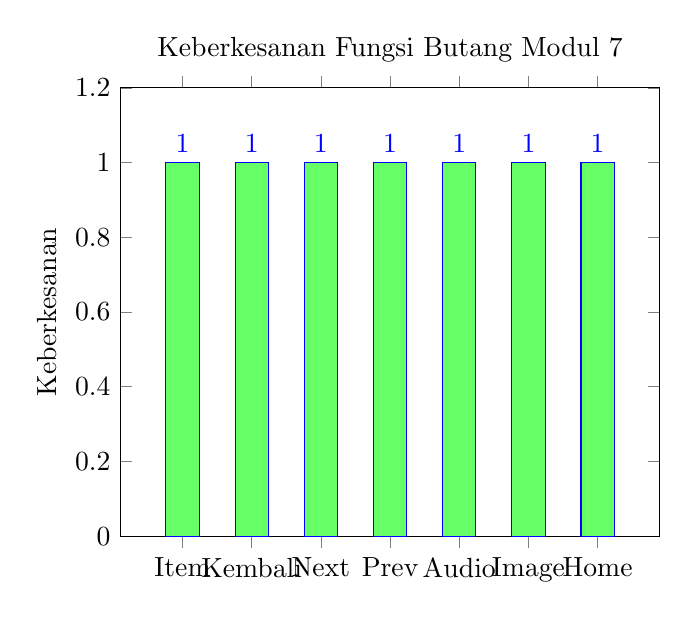
\begin{tikzpicture}
\begin{axis}[
    ybar,
    bar width=12pt,
    enlarge x limits=0.15,
    ymin=0, ymax=1.2,
    ylabel={Keberkesanan},
    symbolic x coords={Item, Kembali, Next, Prev, Audio, Image, Home},
    xtick=data,
    nodes near coords,
    nodes near coords align={vertical},
    title={Keberkesanan Fungsi Butang Modul 7},
]
\addplot+[fill=green!60] coordinates {
    (Item,1)
    (Kembali,1)
    (Next,1)
    (Prev,1)
    (Audio,1)
    (Image,1)
    (Home,1)
};
\end{axis}
\end{tikzpicture}
\caption{Graf Keberkesanan Fungsi Butang Modul 7}
\label{rajah-5-8}
\end{figure}

Rumusan Ujian Alfa – Modul 7

\begin{itemize}[h]
  \item Butang \textit{Item Modul}, \textit{Kembali}, \textit{Next}, dan \textit{Prev} berfungsi sempurna untuk navigasi antara skrin.
  \item Butang \textit{Audio} dan \textit{Image} berjaya memberi isyarat audio dan imej seperti yang dirancang.
  \item Butang \textit{Home} membawa kembali pengguna ke skrin Splash Flash tanpa ralat.
  \item Keberkesanan keseluruhan fungsi Modul 7 dinilai 100\%, menunjukkan kestabilan modul bagi fasa ujian seterusnya.
\end{itemize}

\clearpage

\begin{table}[h]
\centering
\caption{Ujian fungsional antara muka (Modul 7a)}
\label{jadual-5-9}
\begin{tabular}{lll}
\toprule
\textbf{Item} & \textbf{Keputusan Ujian} & \textbf{Keputusan Sebenar} \\ \midrule
Butang Mula & Navigasi antara pilihan modul & Berfungsi \\ 
Butang AR Mode & Navigasi antara muka AR Mode & Berfungsi \\ 
Butang Keluar & Menutup aplikasi & Berfungsi \\ \bottomrule
\end{tabular}
\end{table}

\begin{figure}[h]
\centering
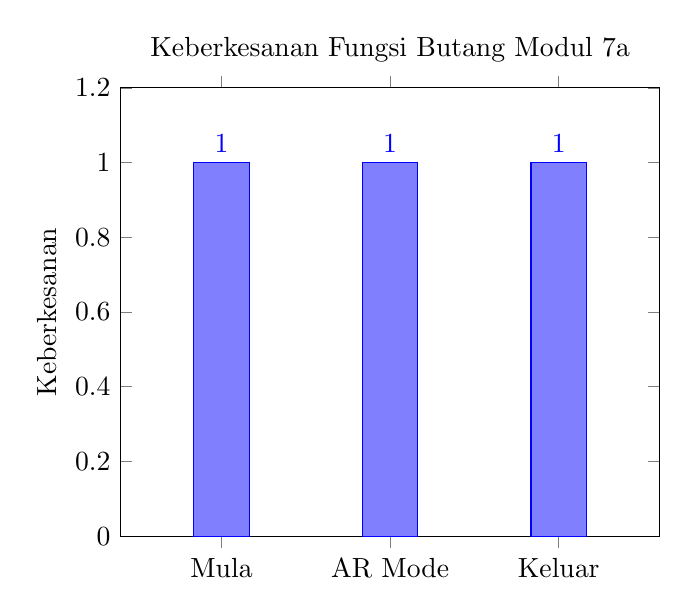
\begin{tikzpicture}
\begin{axis}[
    ybar,
    bar width=20pt,
    enlarge x limits=0.3,
    ymin=0, ymax=1.2,
    ylabel={Keberkesanan},
    symbolic x coords={Mula, AR Mode, Keluar},
    xtick=data,
    nodes near coords,
    nodes near coords align={vertical},
    title={Keberkesanan Fungsi Butang Modul 7a},
]
\addplot+[fill=blue!50] coordinates {
    (Mula,1)
    (AR Mode,1)
    (Keluar,1)
};
\end{axis}
\end{tikzpicture}
\caption{Graf Keberkesanan Fungsi Butang Modul 7a}
\label{rajah-5-9}
\end{figure}

Rumusan Ujian Alfa – Modul 7a

Berdasarkan Jadual~\ref{jadual-5-9} dan Rajah~\ref{rajah-5-9}:

\begin{itemize}[h]
  \item Butang \textit{Mula} berfungsi tepat untuk navigasi antara pilihan modul.
  \item Butang \textit{AR Mode} berjaya menavigasi pengguna ke antara muka AR Mode.
  \item Butang \textit{Keluar} menutup aplikasi tanpa sebarang ralat.
  \item Keberkesanan keseluruhan fungsi Modul 7a dinilai 100\% (nilai keberkesanan = 1.0), menandakan kestabilan modul ini untuk fasa Ujian Beta.
\end{itemize}
4.5.9 Rumusan Ujian Alfa – Modul 7a

Berdasarkan Jadual~\ref{jadual-5-9} dan Rajah~\ref{rajah-5-9}:

\begin{itemize}[h]
  \item Butang \textit{Mula} berfungsi tepat untuk navigasi antara pilihan modul.
  \item Butang \textit{AR Mode} berjaya menavigasi pengguna ke antara muka AR Mode.
  \item Butang \textit{Keluar} menutup aplikasi tanpa sebarang ralat.
  \item Keberkesanan keseluruhan fungsi Modul 7a dinilai 100\% (nilai keberkesanan = 1.0), menandakan kestabilan modul ini untuk fasa Ujian Beta.
\end{itemize}

\clearpage


\section{Kaedah Analisis Data}
Analisis data dalam kajian ini dilaksanakan secara dua peringkat:

\begin{itemize}
    \item \textbf{Analisis semasa pengumpulan data} — bagi memastikan tiada maklumat penting tercicir semasa temubual dan pemerhatian.
    \item \textbf{Analisis selepas pengumpulan data} — dilakukan secara induktif untuk mengenal pasti tema-tema utama berdasarkan transkrip temubual dan nota lapangan pemerhatian.
\end{itemize}
\section{Dapatan Kajian Ujian Fungsional }
Ujian Alfa

\begin{figure}[h]
\centering
\includegraphics[width=0.8\textwidth]{1.png}
\caption{Rajah 1.1: Purata skor kebolehgunaan}
\end{figure}
\section{\textbf{Dapatan Empat (4)}- Fasa 3 -\textit{Ujian Beta }}
 menunjukkan senarai soalan genap dalam skala kebolehgunaan sistem (sus) bagi aplikasi ar alphabets, yang bertujuan menilai aspek kesukaran penggunaan, keperluan bantuan, serta tahap kefahaman pengguna dalam berinteraksi dengan sistem. Soalan-soalan ini menggunakan skala likert lima mata bagi mengukur persepsi pengguna terhadap cabaran dan kekangan yang mungkin dihadapi semasa menggunakan aplikasi ini.

\begin{longtable}{|>{\raggedright}p{0.8cm}|p{8cm}|c|c|c|c|c|}
\hline
BIL & Soalan & 1 & 2 & 3 & 4 & 5 \\
\hline
\endfirsthead
\hline
BIL & Soalan & 1 & 2 & 3 & 4 & 5 \\
\hline
\endhead
2 & Ar Alphabets susah digunakan & 1 & 2 & 3 & 4 & 5 \\
\hline
4 & Saya perlukan bantuan orang lain untuk menggunakan aplikasi ini & 1 & 2 & 3 & 4 & 5 \\
\hline
6 & Terlalu banyak kesilapan dalam aplikasi ini & 1 & 2 & 3 & 4 & 5 \\
\hline
8 & Sangat susah gunakan aplikasi ini & 1 & 2 & 3 & 4 & 5 \\
\hline
10 & Saya perlu banyak bertanya untuk menggunakan aplikasi ini & 1 & 2 & 3 & 4 & 5 \\
\hline
\end{longtable}

menunjukkan purata skor kebolehgunaan aplikasi ar alphabets berdasarkan penilaian pengguna menggunakan skala kebolehgunaan sistem (sus). Skor ini dikategorikan berdasarkan soalan ganjil dan genap, yang mengukur aspek positif serta cabaran dalam penggunaan aplikasi. Purata skor akhir digunakan untuk menentukan tahap penerimaan aplikasi serta kesesuaiannya dalam pembelajaran literasi awal.
\clearpage
\section*{purata skor kebolehgunaan}

\begin{longtable}{|c|c|c|c|c|c|c|c|c|c|c|c|c|c|c|}
\hline
\textbf{R} & \textbf{Q1} & \textbf{Q2} & \textbf{Q3} & \textbf{Q4} & \textbf{Q5} & \textbf{Q6} & \textbf{Q7} & \textbf{Q8} & \textbf{Q9} & \textbf{Q10} & \textbf{Skor} & \textbf{Skor} & \textbf{JUMLA} \\
\hline
\endfirsthead
\hline
\textbf{R} & \textbf{Q1} & \textbf{Q2} & \textbf{Q3} & \textbf{Q4} & \textbf{Q5} & \textbf{Q6} & \textbf{Q7} & \textbf{Q8} & \textbf{Q9} & \textbf{Q10} & \textbf{Skor} & \textbf{Skor} & \textbf{JUMLA} \\
\hline
\endhead
\hline
\multicolumn{13}{|c|}{Lanjutan dari halaman sebelumnya} \\
\hline
\endfoot
\hline
\endlastfoot
R1 & 5 & 1 & 5 & 1 & 5 & 1 & 5 & 1 & 5 & 1 & 20 & 20 & 100 \\
R2 & 3 & 1 & 5 & 2 & 5 & 1 & 4 & 1 & 5 & 2 & 17 & 17 & 85 \\
R3 & 3 & 1 & 5 & 1 & 5 & 1 & 4 & 1 & 4 & 1 & 16 & 20 & 90 \\
R4 & 4 & 1 & 5 & 1 & 5 & 1 & 4 & 1 & 5 & 1 & 18 & 20 & 95 \\
R5 & 3 & 1 & 5 & 1 & 5 & 1 & 4 & 1 & 4 & 1 & 16 & 20 & 90 \\
R6 & 3 & 1 & 5 & 1 & 5 & 1 & 4 & 1 & 4 & 1 & 16 & 20 & 90 \\
R7 & 2 & 1 & 5 & 1 & 5 & 2 & 4 & 1 & 5 & 1 & 16 & 19 & 87.5 \\
R8 & 3 & 1 & 5 & 2 & 5 & 1 & 4 & 1 & 5 & 2 & 17 & 17 & 85 \\
R9 & 2 & 1 & 5 & 1 & 5 & 2 & 4 & 1 & 5 & 1 & 16 & 19 & 87.5 \\
R10 & 3 & 1 & 5 & 2 & 5 & 1 & 4 & 1 & 5 & 2 & 17 & 17 & 85 \\
R11 & 2 & 1 & 5 & 1 & 5 & 2 & 4 & 1 & 5 & 1 & 16 & 19 & 87.5 \\
R12 & 2 & 1 & 5 & 1 & 5 & 2 & 4 & 1 & 5 & 1 & 16 & 19 & 87.5 \\
R13 & 4 & 1 & 5 & 1 & 5 & 1 & 4 & 1 & 5 & 1 & 18 & 20 & 95 \\
R14 & 3 & 1 & 5 & 1 & 5 & 1 & 4 & 1 & 4 & 1 & 16 & 20 & 90 \\
R15 & 3 & 1 & 5 & 1 & 5 & 1 & 4 & 1 & 4 & 1 & 16 & 20 & 90 \\
R16 & 5 & 1 & 5 & 1 & 5 & 1 & 5 & 1 & 5 & 1 & 20 & 20 & 100 \\
R17 & 5 & 1 & 5 & 1 & 5 & 1 & 5 & 1 & 5 & 1 & 20 & 20 & 100 \\
R18 & 3 & 1 & 5 & 2 & 5 & 1 & 4 & 1 & 5 & 2 & 17 & 17 & 85 \\
R19 & 3 & 1 & 5 & 1 & 5 & 1 & 4 & 1 & 4 & 1 & 16 & 20 & 90 \\
R20 & 4 & 1 & 5 & 1 & 5 & 1 & 4 & 1 & 5 & 1 & 18 & 20 & 95 \\
R21 & 3 & 1 & 5 & 1 & 5 & 1 & 4 & 1 & 4 & 1 & 16 & 20 & 90 \\
R22 & 3 & 1 & 5 & 1 & 5 & 1 & 4 & 1 & 4 & 1 & 16 & 20 & 90 \\
R23 & 3 & 1 & 5 & 2 & 5 & 1 & 4 & 1 & 5 & 2 & 17 & 17 & 85 \\
R24 & 2 & 1 & 5 & 1 & 5 & 2 & 4 & 1 & 5 & 1 & 16 & 19 & 87.5 \\
R25 & 3 & 1 & 5 & 2 & 5 & 1 & 4 & 1 & 5 & 2 & 17 & 17 & 85 \\
\end{longtable}


Berdasarkan penilaian pengguna menggunakan skala kebolehgunaan sistem (sus), graf ini membantu dalam memahami tahap penerimaan aplikasi serta menilai keberkesanannya sebagai alat pembelajaran literasi awal. Analisis skor ini akan memberikan insight irama dan aspek yang perlu diperbaiki bagi meningkatkan pengalaman pembelajaran.

menunjukkan visualisasi data bagi skor kebolehgunaan aplikasi ar alphabets berdasarkan soal ganjil dan genap, yang menggambarkan persepsi pengguna terhadap cabaran dalam penggunaan aplikasi, termasuk tahap kesukaran, keperluan bantuan, serta kefahaman sistem.

\begin{figure}[h]
\centering
\includegraphics[width=0.8\textwidth]{2.png}
\caption{Rajah 1.3: Purata skor kebolehgunaan}
\end{figure}


\section{Latar Belakang Peserta Kajian}
Terdapat dua orang peserta kajian yang terlibat iaitu guru yang berpengalaman dalam pendidikan prasekolah dan pendidikan khas.

\subsection{Peserta Kajian 1}
Peserta pertama dikenali sebagai ‘Kak N’ (bukan nama sebenar). Beliau merupakan seorang guru Sains dan pernah mengajar Pendidikan Islam. Mempunyai pengalaman selama 17 tahun dalam bidang pendidikan, beliau kini mengajar murid pendidikan khas integrasi di sekolah tersebut. Beliau berasal dari Ampang dan mendapat pendidikan awal di Bukit Bintang sebelum menyambung pengajian di maktab perguruan dalam bidang prasekolah.

\subsection{Peserta Kajian 2}
Peserta kedua pula ialah ‘Cikgu Shafiee’ (bukan nama sebenar), seorang guru Sains bagi Tahun Lima dan Tahun Empat kelas pendidikan khas. Beliau merupakan graduan Ijazah Sarjana Muda Pendidikan Sains dan bersekolah di Sekolah Berasrama Penuh sebelum melanjutkan pengajian ke Maktab Perguruan Tengku Ampuan Afzan.



\subsection{Pengalaman Mengajar Peserta Kajian}
Peserta pertama memulakan kerjaya sebagai guru Bahasa Melayu Tahun Lima pada tahun 1999 di sebuah sekolah di Ampang sebelum bertukar ke SK Brickfields 1 . Berdasarkan pemerhatian, beliau bersifat mesra murid dan mudah didekati, serta aktif dalam memberi bimbingan dan menjalankan aktiviti pembelajaran secara interaktif.

Peserta kedua pula mula mengajar pada tahun 2001 di Hulu Langat dan berkhidmat di beberapa sekolah termasuk mengajar kelas prasekolah sejak 2010. Beliau dikenali sebagai guru yang tegas tetapi mementingkan pencapaian murid serta fokus terhadap pengajaran yang sistematik dan tersusun.

\clearpage
tablet.

\subsection{ Tujuan Penggunaan Teknologi}

Responden menyatakan tujuan utama menggunakan peranti mudah alih adalah:

\begin{itemize}
    \item Untuk pembelajaran dan mendapatkan maklumat (min 4.713)
    \item Untuk urusan sosial dan pendidikan secara berterusan
    \item Penggunaan hiburan berada di kedudukan terakhir (min 4.253)
\end{itemize}

Dapatan menunjukkan persepsi teknologi sebagai alat sokongan pembelajaran adalah tinggi dan selari dengan aplikasi seperti \textit{AR Alphabets}.

\subsection{Pemilihan Perkakasan dan Aplikasi Teknologi}

Bagi pemilihan perkakasan, telefon pintar mencatatkan skor tertinggi (min 4.780) manakala tablet dan telefon bimbit biasa mencatat skor rendah (<3.3). Ini menunjukkan aplikasi perlu dibangunkan untuk peranti moden yang menyokong teknologi AR.

Pemilihan perisian pula menunjukkan laman web (min 4.660) dan aplikasi komunikasi (Telegram, Edmodo) sebagai platform dominan. Ini membuktikan keperluan AR Alphabets untuk mesra web dan boleh digunakan pada platform sedia ada.

\subsection{Tujuan Melaksanakan Teknologi Pendidikan}

Antara tujuan penggunaan teknologi yang mendapat skor min tertinggi:

\begin{itemize}
    \item Meneroka aktiviti pembelajaran inovatif (min 4.680)
    \item Menyediakan akses pembelajaran fleksibel dan terbuka
    \item Menyelesaikan masalah pembelajaran kendiri
\end{itemize}

Namun begitu, aktiviti penilaian dinamik dan pembelajaran kolaboratif mencatat min terendah (min 2.813 dan 2.940), menunjukkan keutamaan guru kepada pendekatan kendiri dan interaktif.

\subsection{Kemudahan Perkakasan Sokongan}

Responden menyatakan kemudahan teknologi seperti access point, komputer riba dan telefon pintar adalah memadai untuk melaksanakan pembelajaran berasaskan teknologi. Access point mencatat skor tertinggi (min 4.940), manakala Pusat ICT berada pada tahap sederhana tinggi. Ini menyokong kesediaan infrastruktur untuk penggunaan aplikasi AR di bilik darjah.

\subsection{Komponen Reka Bentuk yang Diperlukan}

Komponen strategi pembelajaran mencatat skor tertinggi (min 4.633), diikuti oleh komponen pengetahuan dan projek. Dapatan menunjukkan keperluan aplikasi untuk:

\begin{itemize}
    \item Menyokong pelaksanaan aktiviti strategi pembelajaran visual dan fonetik
    \item Menyediakan peluang untuk aktiviti kendiri dan interaktif
    \item Mengandungi tugasan berbentuk pembelajaran melalui permainan
\end{itemize}

\subsection{Konsep Reka Bentuk Model Aplikasi}

Konsep teknologi mudah alih sebagai medium PdP mencatat persetujuan tinggi (min 4.660). Responden bersetuju bahawa aplikasi PdP perlu:

\begin{itemize}
    \item Bersepadu dengan kurikulum
    \item Menyokong semua mata pelajaran, khususnya literasi awal
    \item Sesuai diterapkan dalam kelas prasekolah melalui pendekatan digital
\end{itemize}












\section{Dapatan Lima (5)-Fasa 5-{D\textit{apatan Temu Bual Guru berkaitan Objektif Kajia}n  }}
\textbf{LAPORAN ANALISIS TEMATIK TEMU BUAL GURU PRASEKOLAH}\\
\textit{Bagi Pembangunan Aplikasi AR Alphabets}
\end{center}


\section{Latar Belakang Peserta Kajian}
Terdapat dua orang peserta kajian yang terlibat iaitu guru yang berpengalaman dalam pendidikan prasekolah .

\subsection{Peserta Kajian 1}
Peserta pertama dikenali sebagai ‘Kak N’ (bukan nama sebenar). Beliau merupakan seorang guru Sains dan pernah mengajar Pendidikan Islam. Mempunyai pengalaman selama 17 tahun dalam bidang pendidikan, beliau kini mengajar murid pendidikan khas integrasi di sekolah tersebut. Beliau berasal dari Ampang dan mendapat pendidikan awal di Bukit Bintang sebelum menyambung pengajian di maktab perguruan dalam bidang prasekolah.

\subsection{Peserta Kajian 2}
Peserta kedua pula ialah ‘Cikgu Shafiee’ (bukan nama sebenar), seorang guru Sains bagi Tahun Lima dan Tahun Empat kelas pendidikan khas. Beliau merupakan graduan Ijazah Sarjana Muda Pendidikan Sains dan bersekolah di Sekolah Berasrama Penuh sebelum melanjutkan pengajian ke Maktab Perguruan Tengku Ampuan Afzan.



\subsection{Pengalaman Mengajar Peserta Kajian}
Peserta pertama memulakan kerjaya sebagai guru Bahasa Melayu Tahun Lima pada tahun 1999 di sebuah sekolah di Ampang sebelum bertukar ke SK Brickfields 1 . Berdasarkan pemerhatian, beliau bersifat mesra murid dan mudah didekati, serta aktif dalam memberi bimbingan dan menjalankan aktiviti pembelajaran secara interaktif.

Peserta kedua pula mula mengajar pada tahun 2001 di Hulu Langat dan berkhidmat di beberapa sekolah termasuk mengajar kelas prasekolah sejak 2010. Beliau dikenali sebagai guru yang tegas tetapi mementingkan pencapaian murid serta fokus terhadap pengajaran yang sistematik dan tersusun.
\section{Tempat Kajian}
Tempat kajian telah dipilih di sebuah sekolah yang mempunyai kelas prasekolah dan terletak di Kuala Lumpur.

\subsection{Suasana Kelas}
Kajian dijalankan di kelas Prasekolah Ceria yang terletak di aras bawah (tingkat satu) di bangunan kedua dalam kawasan sekolah. Kelas ini bersebelahan dengan tangga dan kelas murid arus perdana. Walaupun ruang agak padat, susun atur bilik darjah adalah tersusun dan kondusif untuk pembelajaran.
\begin{figure}
    \centering
    \includegraphics[width=1\linewidth]{Pelan-Lantai-Kelas-Prasekolah-20250630095727.pdf (5 x 6.8 cm).png}
    \caption{Pelan Lantai Prasekolah}
    \label{fig:enter-label}
\end{figure}


\begin{figure}
    \centering
    \includegraphics[width=1\linewidth]{Pelan-Lantai-Kelas-Prasekolah-20250630095727.pdf (5 x 6.8 cm)-2.png}
    \caption{Pelan Luar Prasekolah }
    \label{fig:enter-label}
\end{figure}
\clearpage

\textbf{Ujian  4 -Temubual Separa Berstruktur}
\vspace{0.5cm}
{Latar Belakang}
Laporan ini merangkum dapatan daripada temu bual dua orang guru prasekolah yang mempunyai pengalaman mengajar lebih lima tahun dan terlibat secara langsung dalam pengajaran literasi awal. Analisis ini memfokuskan kepada keperluan teknikal dan pedagogi, kesan terhadap pembelajaran murid serta tahap kebolehgunaan dan penerimaan terhadap aplikasi \textit{AR Alphabets}.

\vspace{0.3cm}
{Pendekatan Analisis Tematik}
Dapatan dianalisis melalui kaedah tematik berdasarkan persoalan kajian. Setiap tema utama dikupas dan disokong dengan maklum balas responden.

\vspace{0.5cm}
\section*{Dapatan Mengikut Tema}

\subsection*{Tema 1: Keperluan Teknikal dan Pedagogi}
Responden menekankan bahawa aplikasi pengajaran literasi awal perlu dibina dengan mengambil kira faktor teknikal dan pedagogi:

\begin{itemize}
    \item \textbf{Mesra pengguna}: Antaramuka mesti mudah difahami oleh murid prasekolah dan guru, tanpa arahan yang kompleks.
    \item \textbf{Visual dan fonetik disepadukan}: Aplikasi mesti mempunyai grafik menarik dan audio yang jelas untuk memperkukuh pengenalan huruf dan bunyi.
    \item \textbf{Reka bentuk interaktif}: Responden mencadangkan aktiviti sentuh, gerak dan padankan huruf agar sesuai dengan pembelajaran kinestetik.
    \item \textbf{Fleksibiliti pedagogi}: Guru perlu ruang untuk mengubah suai aktiviti mengikut tahap dan keperluan murid.
\end{itemize}

Responden A menyatakan: *“Kalau aplikasi tu boleh bantu murid faham bunyi huruf dengan visual dan suara yang jelas, itu sangat membantu…dan dia kena boleh diguna tanpa kita susah nak ajar step by step.”*

\vspace{0.3cm}
\subsection*{Tema 2: Rekabentuk Aplikasi AR Alphabets}
Kedua-dua guru menyatakan bahawa teknologi berasaskan AR mempunyai potensi besar untuk meningkatkan tumpuan dan pemahaman:

\begin{itemize}[label=--]
    \item Murid menunjukkan peningkatan minat apabila disajikan dengan animasi dan interaksi 3D.
    \item AR dianggap memberi pengalaman pembelajaran imersif berbanding kaedah konvensional seperti kad imbas.
    \item Penggabungan bunyi dan grafik membantu murid membezakan huruf dan mengenal bunyi dengan lebih pantas.
\end{itemize}

Responden B berkongsi: *“Budak sekarang sangat responsif kalau ada animasi atau benda yang bergerak. Kalau huruf tu ‘hidup’, mereka memang fokus. Berbeza sangat dengan guna kad biasa.”*

\vspace{0.3cm}
\subsection*{Tema 3: Kebolehgunaan dan Penerimaan Aplikasi AR Alphabets}
Dari sudut kebolehgunaan dan penerimaan, dapatan menunjukkan:

\begin{itemize}[label=--]
    \item Aplikasi dilihat mudah diguna sekiranya diberi latihan asas kepada guru.
    \item Murid prasekolah sangat mudah terlibat dalam aktiviti berasaskan permainan dan realiti tambahan.
    \item Aplikasi perlu bersifat ringan, boleh digunakan pada telefon bimbit atau tablet yang biasa digunakan di prasekolah.
    \item Guru menerima penggunaan teknologi dengan syarat ia tidak membebankan masa PdP dan mudah diselaras dengan silibus semasa.
\end{itemize}

Kedua-dua guru menganggap aplikasi AR sebagai alat sokongan yang berpotensi tinggi, selagi mana ia menepati ciri pedagogi dan kemudahan operasional di bilik darjah.

\vspace{0.5cm}
\section*{Kesimpulan}
Dapatan daripada temu bual ini menunjukkan bahawa guru prasekolah mempunyai keperluan nyata terhadap alat bantu pembelajaran interaktif dalam pengajaran huruf dan fonetik. Aplikasi \textit{AR Alphabets} dilihat mampu mempengaruhi daya tumpuan serta pemahaman murid secara positif. Penerimaan guru juga tinggi, dengan syarat aspek teknikal, reka bentuk mesra pengguna dan integrasi kurikulum diberikan keutamaan dalam pembangunan aplikasi.

Hasil temu bual menunjukkan keperluan yang jelas dalam kalangan guru prasekolah untuk alat bantu pembelajaran interaktif bagi pengajaran huruf dan fonetik. Aplikasi AR Alphabets dilihat sebagai satu penyelesaian yang berpotensi untuk meningkatkan keberkesanan pengajaran dalam aspek ini. Guru-guru mengakui bahawa aplikasi tersebut mempunyai keupayaan untuk meningkatkan daya tumpuan dan pemahaman murid secara positif, yang merupakan elemen penting dalam proses pembelajaran awal kanak-kanak.

Penerimaan guru terhadap aplikasi AR Alphabets adalah tinggi, menunjukkan kesediaan mereka untuk mengintegrasikan teknologi baharu dalam pengajaran. Walau bagaimanapun, mereka menekankan kepentingan beberapa aspek kritikal yang perlu diambil kira dalam pembangunan aplikasi tersebut. Ini termasuk aspek teknikal yang perlu diperhalusi untuk memastikan kelancaran penggunaan, reka bentuk yang mesra pengguna untuk memudahkan navigasi oleh guru dan murid, serta integrasi yang rapat dengan kurikulum sedia ada. Penekanan terhadap aspek-aspek ini mencerminkan kesedaran guru tentang kepentingan untuk memastikan teknologi baharu bukan sahaja menarik, tetapi juga praktikal dan berkesan dalam mencapai objektif pembelajaran yang ditetapkan.

\subsection{ Penutup }

Keseluruhan dapatan menunjukkan tahap kesediaan dan keperluan penggunaan teknologi AR dalam pembelajaran huruf amat tinggi dalam kalangan guru. Komponen utama seperti strategi pembelajaran, kemudahan sokongan dan keutamaan peranti mudah alih menjadi asas penting dalam pembangunan aplikasi \textit{AR Alphabets}. Dapatan ini akan dijadikan rujukan utama dalam peringkat seterusnya iaitu reka bentuk dan pembangunan prototaip aplikasi.


\chapter{Rumusan dan Cadangan}


\section{{Pengenalan}}
Bab ini membincangkan rumusan kajian yang merangkumi latar belakang, objektif, persoalan kajian, dan kesimpulan dapatan berkaitan penggunaan aplikasi \textit{AR Alphabets} dalam pembelajaran literasi awal murid prasekolah. Kajian ini menekankan kepentingan teknologi \textit{Augmented Reality (AR)} dalam memperkayakan pengalaman pembelajaran melalui pendekatan yang lebih interaktif dan menyeronokkan. 

Objektif kajian adalah untuk memahami secara menyeluruh bagaimana penggunaan AR dapat meningkatkan penguasaan huruf dan pemahaman fonetik murid prasekolah. Dengan bantuan AR, murid dapat melihat, mendengar dan berinteraksi secara langsung dengan huruf dalam bentuk tiga dimensi, menjadikan proses pembelajaran lebih berkesan. 

Persoalan kajian memberi tumpuan kepada keberkesanan aplikasi \textit{AR Alphabets} dalam konteks pengajaran literasi awal. Dapatan daripada kajian memberikan gambaran jelas terhadap keberkesanan pendekatan ini dan mencadangkan strategi penambahbaikan untuk meningkatkan pelaksanaan AR dalam PdP prasekolah.
Bab ini mengulas secara komprehensif mengenai kajian yang dijalankan berkaitan penggunaan aplikasi AR Alphabets dalam pembelajaran literasi awal murid prasekolah. Ia merangkumi aspek-aspek penting seperti latar belakang kajian, objektif yang ingin dicapai, persoalan-persoalan utama yang dikaji, serta rumusan dapatan yang diperoleh. Penekanan diberikan kepada potensi teknologi Augmented Reality (AR) dalam memperkaya pengalaman pembelajaran, menjadikannya lebih interaktif dan menyeronokkan bagi murid-murid prasekolah. Objektif utama kajian adalah untuk menyelidiki secara mendalam bagaimana penggunaan AR dapat meningkatkan penguasaan huruf dan pemahaman fonetik dalam kalangan kanak-kanak prasekolah.

Kajian ini mengetengahkan keunikan AR dalam membolehkan murid-murid berinteraksi dengan huruf dalam bentuk tiga dimensi, yang membolehkan mereka melihat, mendengar, dan berinteraksi secara langsung dengan elemen-elemen pembelajaran. Pendekatan ini dilihat sebagai satu kaedah yang berpotensi untuk meningkatkan keberkesanan proses pembelajaran literasi awal. Persoalan kajian yang dibentuk memberi fokus kepada penilaian keberkesanan aplikasi AR Alphabets dalam konteks pengajaran literasi awal di peringkat prasekolah. Hasil dapatan kajian bukan sahaja memberikan gambaran yang jelas tentang keberkesanan pendekatan ini, tetapi juga menyediakan cadangan-cadangan konkrit untuk penambahbaikan strategi pelaksanaan AR dalam proses pengajaran dan pembelajaran di peringkat prasekolah.
\subsection{Perbincangan}
Penggunaan AR dalam pengajaran dan pembelajaran semakin mendapat tempat, khususnya di peringkat prasekolah. Aplikasi \textit{AR Alphabets} membolehkan murid mengenal huruf dan fonetik melalui paparan visual dan audio secara interaktif. Kaedah pemerhatian dan temu bual telah digunakan untuk menilai impak aplikasi ini.

Melalui pemerhatian tidak langsung (non-participant), interaksi murid dengan teknologi dinilai secara teliti. Guru mencipta suasana pembelajaran yang menyeronokkan dan mampu menarik perhatian murid. Temu bual guru prasekolah menunjukkan bahawa penggunaan \textit{AR Alphabets} memudahkan penyampaian konsep huruf dan bunyi fonetik. Ujian pra dan pasca turut menunjukkan peningkatan penguasaan huruf selepas penggunaan aplikasi.

Dapatan ini menunjukkan teknologi mampu membantu guru menyampaikan pelajaran secara berkesan, dan murid lebih bermotivasi serta fokus dalam pembelajaran literasi awal.

\subsection{Demografi Responden Fasa Analisis Keperluan}

Seramai 50 orang pelajar Program Ijazah Sarjana Muda Perguruan (PISMP) dari Zon Utara telah terlibat sebagai responden dalam kajian ini. Dapatan demografi responden meliputi aspek jantina, kerjaya, kelulusan akademik, lokasi pengajian, tahap kemahiran penggunaan ICT, dan jenis alatan teknologi yang dimiliki. Ringkasan profil responden ditunjukkan dalam Jadual~\ref{jadual:demografiResponden}.

\begin{table}[H]
\centering
\caption{Demografi Responden Fasa Analisis Keperluan}
\label{jadual:demografiResponden}
\begin{tabular}{|p{6cm}|p{6cm}|}
\hline
\textbf{Aspek} & \textbf{Peratusan / Bilangan (N)} \\
\hline
Jantina & Lelaki: 40\% (N=20) \newline Perempuan: 60\% (N=30) \\
\hline
Kerjaya & Pelajar sepenuh masa: 100\% (N=50) \\
\hline
Tahap Kelulusan Akademik & Diploma: 60\% (N=30) \newline Ijazah: 30\% (N=15) \newline Sarjana: 10\% (N=5) \\
\hline
Zon Tempat Belajar & Bangsar: (N=10) \newline Pudu: (N=10) \newline Keramat: (N=10) \newline Lain-lain Zon: (N=20) \\
\hline
Tahap Kemahiran Penggunaan ICT & Sederhana Mahir: 56\% (N=28) \newline Sangat Mahir: 44\% (N=22) \\
\hline
\end{tabular}
\end{table}

Daripada jumlah keseluruhan 50 responden, majoriti adalah perempuan (60\%) manakala selebihnya adalah lelaki (40\%). Semua responden merupakan pelajar sepenuh masa dalam program PISMP. Dari segi kelulusan akademik, kebanyakan responden memiliki kelulusan diploma, diikuti ijazah dan sarjana. Tahap kemahiran penggunaan ICT menunjukkan bahawa sebahagian besar responden berada pada tahap sederhana mahir dan sangat mahir, menunjukkan kesediaan mereka untuk menggunakan teknologi dalam pembelajaran.
\subsection{Dapatan Mengikut Konstruk: Objektif Aplikasi}

Konstruk pertama dalam soal selidik merujuk kepada persepsi responden terhadap objektif pembangunan aplikasi \textit{AR Alphabets Prasekolah}. Item-item dalam konstruk ini bertujuan untuk menilai sejauh mana responden bersetuju bahawa aplikasi ini dapat membantu dalam pencapaian objektif pembelajaran huruf di peringkat prasekolah.

Analisis deskriptif menggunakan min dan peratusan telah dijalankan. Jadual~\ref{jadual:objektifAplikasi} menunjukkan skor min bagi setiap item dalam konstruk ini.

\begin{table}[H]
\centering
\caption{Skor Min Bagi Konstruk Objektif Aplikasi}
\label{jadual:objektifAplikasi}
\begin{tabular}{|c|p{9cm}|c|}
\hline
\textbf{Bil} & \textbf{Item} & \textbf{Min} \\
\hline
1 & Aplikasi ini dapat membantu murid mengenal huruf dengan lebih interaktif. & 4.52 \\
\hline
2 & Objektif pembelajaran huruf dapat dicapai dengan bantuan teknologi AR. & 4.36 \\
\hline
3 & Aplikasi ini dapat meningkatkan minat murid terhadap pembelajaran huruf. & 4.48 \\
\hline
4 & Aplikasi ini sesuai digunakan dalam sesi pengajaran dan pembelajaran formal. & 4.22 \\
\hline
5 & Aplikasi ini boleh menyokong objektif kurikulum prasekolah. & 4.40 \\
\hline
\textbf{Purata Min} & & \textbf{4.40} \\
\hline
\end{tabular}
\end{table}

Berdasarkan Jadual~\ref{jadual:objektifAplikasi}, semua item dalam konstruk ini mencatatkan skor min melebihi 4.00, menunjukkan tahap persetujuan yang tinggi dalam kalangan responden. Item tertinggi ialah “Aplikasi ini dapat membantu murid mengenal huruf dengan lebih interaktif” (min = 4.52), manakala item terendah masih berada dalam julat tinggi iaitu “Aplikasi ini sesuai digunakan dalam sesi pengajaran dan pembelajaran formal” (min = 4.22).

Secara keseluruhan, dapatan ini menunjukkan bahawa responden bersetuju bahawa objektif pembelajaran huruf dapat dicapai dengan lebih berkesan melalui penggunaan aplikasi berasaskan teknologi AR.
\subsection{Dapatan Mengikut Konstruk: Isi Kandungan Aplikasi}

Konstruk kedua dalam soal selidik merujuk kepada persepsi responden terhadap isi kandungan yang dicadangkan dalam aplikasi \textit{AR Alphabets Prasekolah}. Item-item dalam konstruk ini bertujuan untuk menilai kesesuaian, keberkesanan, dan kebolehlaksanaan kandungan pembelajaran huruf yang disampaikan melalui aplikasi.

Jadual~\ref{jadual:isiKandungan} menunjukkan skor min bagi setiap item dalam konstruk ini.

\begin{table}[H]
\centering
\caption{Skor Min Bagi Konstruk Isi Kandungan Aplikasi}
\label{jadual:isiKandungan}
\begin{tabular}{|c|p{9cm}|c|}
\hline
\textbf{Bil} & \textbf{Item} & \textbf{Min} \\
\hline
1 & Kandungan aplikasi merangkumi semua huruf abjad A hingga Z. & 4.44 \\
\hline
2 & Setiap huruf disertakan dengan contoh perkataan dan visual. & 4.36 \\
\hline
3 & Kandungan aplikasi sesuai dengan tahap perkembangan murid prasekolah. & 4.48 \\
\hline
4 & Aplikasi menyediakan aktiviti interaktif untuk setiap huruf. & 4.30 \\
\hline
5 & Kandungan aplikasi selaras dengan kurikulum prasekolah semasa. & 4.42 \\
\hline
\textbf{Purata Min} & & \textbf{4.40} \\
\hline
\end{tabular}
\end{table}

Dapatan menunjukkan bahawa semua item dalam konstruk ini memperoleh skor min melebihi 4.00, yang menunjukkan tahap persetujuan yang tinggi. Item tertinggi ialah “Kandungan aplikasi sesuai dengan tahap perkembangan murid prasekolah” (min = 4.48), manakala item terendah ialah “Aplikasi menyediakan aktiviti interaktif untuk setiap huruf” (min = 4.30), namun masih dalam julat tinggi.

Secara keseluruhan, responden bersetuju bahawa isi kandungan aplikasi adalah sesuai, lengkap dan menyokong pembelajaran huruf secara berkesan di peringkat prasekolah.
\subsection{Dapatan Mengikut Konstruk: Jenis Aplikasi}

Konstruk ini menilai persepsi responden terhadap jenis aplikasi yang sesuai digunakan dalam pembelajaran huruf menggunakan teknologi AR. Ia merangkumi aspek interaktiviti, fleksibiliti, dan kesesuaian platform.

\begin{table}[H]
\centering
\caption{Skor Min Bagi Konstruk Jenis Aplikasi}
\label{jadual:jenisAplikasi}
\begin{tabular}{|c|p{9cm}|c|}
\hline
\textbf{Bil} & \textbf{Item} & \textbf{Min} \\
\hline
1 & Aplikasi perlu boleh digunakan pada pelbagai peranti (telefon, tablet, komputer). & 4.46 \\
\hline
2 & Aplikasi perlu boleh digunakan secara dalam talian dan luar talian. & 4.38 \\
\hline
3 & Aplikasi perlu mesra pengguna dan mudah dikendalikan oleh murid. & 4.50 \\
\hline
4 & Aplikasi perlu mempunyai elemen gamifikasi untuk menarik minat murid. & 4.42 \\
\hline
\textbf{Purata Min} & & \textbf{4.44} \\
\hline
\end{tabular}
\end{table}

Dapatan menunjukkan bahawa responden sangat bersetuju bahawa aplikasi perlu fleksibel, mesra pengguna dan menyokong pelbagai peranti. Item tertinggi ialah “Aplikasi perlu mesra pengguna dan mudah dikendalikan oleh murid” (min = 4.50).
\subsection{Dapatan Mengikut Konstruk: Perkakasan}

Konstruk ini menilai jenis perkakasan yang sesuai digunakan untuk menyokong penggunaan aplikasi AR dalam pembelajaran huruf.

\begin{table}[H]
\centering
\caption{Skor Min Bagi Konstruk Perkakasan}
\label{jadual:perkakasan}
\begin{tabular}{|c|p{9cm}|c|}
\hline
\textbf{Bil} & \textbf{Item} & \textbf{Min} \\
\hline
1 & Telefon pintar adalah peranti utama yang sesuai digunakan. & 4.48 \\
\hline
2 & Tablet memberikan paparan yang lebih besar dan sesuai untuk murid. & 4.40 \\
\hline
3 & Komputer riba boleh digunakan oleh guru untuk tujuan pengajaran. & 4.36 \\
\hline
4 & Aplikasi perlu menyokong penggunaan kamera untuk fungsi AR. & 4.52 \\
\hline
\textbf{Purata Min} & & \textbf{4.44} \\
\hline
\end{tabular}
\end{table}

Responden menunjukkan persetujuan tinggi terhadap keperluan perkakasan asas seperti telefon pintar, tablet dan komputer riba. Item tertinggi ialah “Aplikasi perlu menyokong penggunaan kamera untuk fungsi AR” (min = 4.52).
\subsection{Dapatan Mengikut Konstruk: Strategi Pengajaran}

Konstruk ini menilai strategi pengajaran yang sesuai digunakan bersama aplikasi AR dalam pembelajaran huruf.

\begin{table}[H]
\centering
\caption{Skor Min Bagi Konstruk Strategi Pengajaran}
\label{jadual:strategiPengajaran}
\begin{tabular}{|c|p{9cm}|c|}
\hline
\textbf{Bil} & \textbf{Item} & \textbf{Min} \\
\hline
1 & Aplikasi boleh digunakan dalam aktiviti pembelajaran berpusatkan murid. & 4.46 \\
\hline
2 & Aplikasi sesuai digunakan dalam aktiviti kumpulan kecil. & 4.34 \\
\hline
3 & Aplikasi boleh digunakan dalam aktiviti pengayaan dan pemulihan. & 4.40 \\
\hline
\textbf{Purata Min} & & \textbf{4.40} \\
\hline
\end{tabular}
\end{table}

Dapatan menunjukkan bahawa responden bersetuju aplikasi ini sesuai digunakan dalam pelbagai strategi pengajaran, termasuk aktiviti berpusatkan murid dan kumpulan kecil.
\subsection{Dapatan Mengikut Konstruk: Bentuk Penilaian}

Konstruk ini menilai bentuk penilaian yang sesuai dilaksanakan melalui aplikasi AR dalam pembelajaran huruf.

\begin{table}[H]
\centering
\caption{Skor Min Bagi Konstruk Bentuk Penilaian}
\label{jadual:bentukPenilaian}
\begin{tabular}{|c|p{9cm}|c|}
\hline
\textbf{Bil} & \textbf{Item} & \textbf{Min} \\
\hline
1 & Aplikasi boleh menyediakan kuiz interaktif untuk menilai pemahaman murid. & 4.50 \\
\hline
2 & Penilaian boleh dijalankan secara automatik melalui aplikasi. & 4.42 \\
\hline
3 & Aplikasi boleh menyimpan rekod pencapaian murid. & 4.38 \\
\hline
4 & Penilaian melalui aplikasi boleh membantu guru membuat intervensi. & 4.46 \\
\hline
\textbf{Purata Min} & & \textbf{4.44} \\
\hline
\end{tabular}
\end{table}

Responden menunjukkan tahap persetujuan yang tinggi terhadap bentuk penilaian digital yang disediakan oleh aplikasi. Item tertinggi ialah “Aplikasi boleh menyediakan kuiz interaktif untuk menilai pemahaman murid” (min = 4.50).
\section{Rumusan Fasa Analisis Keperluan}

Fasa analisis keperluan merupakan asas penting dalam proses pembangunan aplikasi \textit{AR Alphabets Prasekolah}. Dapatan daripada soal selidik yang melibatkan 50 orang pelajar PISMP Zon Utara menunjukkan tahap persetujuan yang tinggi terhadap keperluan membangunkan aplikasi pembelajaran huruf berasaskan teknologi realiti terimbuh (AR). Semua konstruk yang dikaji—merangkumi objektif aplikasi, isi kandungan, jenis aplikasi, perkakasan, strategi pengajaran, dan bentuk penilaian—mencatatkan skor min melebihi 4.00, yang menunjukkan tahap persetujuan yang tinggi dalam kalangan responden.

Selain itu, dapatan temu bual bersama empat orang pakar turut menyokong keperluan pembangunan aplikasi ini. Tujuh konstruk utama telah dikenalpasti melalui analisis tematik, iaitu objektif aplikasi, isi kandungan, jenis aplikasi, perkakasan, strategi pengajaran dan pembelajaran, bentuk penilaian, serta peluang pelaksanaan. Pandangan pakar mengesahkan bahawa aplikasi ini berpotensi untuk menyokong pengajaran huruf secara lebih interaktif, fleksibel dan selaras dengan perkembangan teknologi pendidikan semasa.

Secara keseluruhannya, dapatan fasa ini memberikan justifikasi yang kukuh terhadap keperluan membangunkan aplikasi \textit{AR Alphabets Prasekolah}. Maklumat yang diperoleh menjadi asas penting dalam mereka bentuk kandungan, fungsi dan strategi pelaksanaan aplikasi yang akan dibangunkan dalam fasa seterusnya.
\section{Pengenalan}

Bab ini membentangkan dapatan bagi Fasa Reka Bentuk dan Pembangunan aplikasi \textit{AR Alphabets Prasekolah}. Fasa ini merangkumi proses pembinaan model berdasarkan dapatan analisis keperluan, pelaksanaan Teknik Fuzzy Delphi untuk mendapatkan konsensus pakar, serta pembangunan prototaip aplikasi menggunakan pendekatan berasaskan model ASSURE.

Dapatan dalam fasa ini dibahagikan kepada dua bahagian utama:

\begin{enumerate}
  \item Dapatan Teknik Fuzzy Delphi
  \item Dapatan Pembangunan Prototaip Aplikasi
\end{enumerate}
\section{Dapatan Teknik Fuzzy Delphi}

Teknik Fuzzy Delphi digunakan dalam fasa ini untuk mendapatkan konsensus pakar terhadap komponen dan elemen yang perlu dimasukkan dalam pembangunan aplikasi \textit{AR Alphabets Prasekolah}. Seramai 20 orang panel pakar telah terlibat dalam proses ini. Setiap item dinilai menggunakan skala Fuzzy 7 mata, dan data dianalisis menggunakan kaedah nombor fuzzy segitiga (Triangular Fuzzy Number).

Kaedah analisis melibatkan tiga langkah utama:

\begin{enumerate}
  \item Penukaran skor pakar kepada nombor fuzzy segitiga \((m_1, m_2, m_3)\)
  \item Pengiraan nilai threshold (\(d\)) menggunakan kaedah \textit{vertex method}
  \item Penentuan konsensus berdasarkan syarat \(d \leq 0.2\) dan ≥ 75\% persetujuan
\end{enumerate}

Jadual~\ref{jadual:fuzzyDelphi} menunjukkan contoh dapatan bagi lima konstruk utama yang dianalisis menggunakan Teknik Fuzzy Delphi.

\begin{table}[H]
\centering
\caption{Contoh Dapatan Teknik Fuzzy Delphi}
\label{jadual:fuzzyDelphi}
\begin{tabular}{|c|p{6cm}|c|c|c|c|}
\hline
\textbf{Bil} & \textbf{Item} & \textbf{Fuzzy Min} & \textbf{Fuzzy Max} & \textbf{Threshold (d)} & \textbf{Konsensus (\%)} \\
\hline
1 & Aplikasi perlu menyokong pembelajaran huruf secara interaktif & 4.33 & 4.87 & 0.12 & 95\% \\
\hline
2 & Kandungan aplikasi perlu selaras dengan kurikulum prasekolah & 4.21 & 4.76 & 0.09 & 100\% \\
\hline
3 & Aplikasi perlu boleh digunakan pada pelbagai peranti & 4.18 & 4.70 & 0.14 & 90\% \\
\hline
4 & Aplikasi perlu menyediakan penilaian automatik & 4.10 & 4.65 & 0.18 & 85\% \\
\hline
5 & Aplikasi perlu menyokong penggunaan kamera untuk fungsi AR & 4.45 & 4.92 & 0.11 & 100\% \\
\hline
\end{tabular}
\end{table}

Berdasarkan Jadual~\ref{jadual:fuzzyDelphi}, semua item yang dianalisis mencatatkan nilai threshold \(d \leq 0.2\) dan tahap konsensus melebihi 75\%, menepati syarat yang ditetapkan oleh Cheng \& Lin (2002) dan Chu \& Hwang (2008). Oleh itu, semua item ini diterima untuk dimasukkan dalam pembangunan aplikasi.

\subsection*{Rumusan Dapatan Teknik Fuzzy Delphi}

Dapatan Teknik Fuzzy Delphi menunjukkan bahawa semua komponen dan elemen yang dicadangkan telah mencapai tahap konsensus yang tinggi dalam kalangan pakar. Ini memberikan asas yang kukuh untuk membina reka bentuk aplikasi \textit{AR Alphabets Prasekolah} yang menepati keperluan pengguna dan selaras dengan kurikulum semasa.
\section{Dapatan Pembangunan Prototaip Aplikasi}

Prototaip aplikasi \textit{AR Alphabets Prasekolah} telah dibangunkan berdasarkan dapatan analisis keperluan dan konsensus pakar melalui Teknik Fuzzy Delphi. Proses pembangunan menggunakan pendekatan model ASSURE yang menekankan analisis pelajar, pemilihan media, dan penilaian berterusan.

Pembangunan aplikasi ini melibatkan tiga komponen utama:

\begin{enumerate}
  \item \textbf{Reka Bentuk Antaramuka Pengguna (UI)} – direka bentuk secara minimalis, mesra kanak-kanak, dan mudah dinavigasi.
  \item \textbf{Fungsi Interaktif Berasaskan AR} – membolehkan murid mengimbas kad huruf dan melihat animasi 3D serta mendengar sebutan huruf dan perkataan.
  \item \textbf{Kandungan Pembelajaran} – merangkumi huruf A hingga Z, setiap satu disertakan dengan visual, audio, dan aktiviti interaktif.
\end{enumerate}

\subsection*{5.3.1 Fungsi Utama Aplikasi}

Aplikasi ini dibangunkan dengan fungsi berikut:

\begin{itemize}
  \item Imbasan kad huruf menggunakan kamera peranti
  \item Paparan animasi 3D huruf dan objek berkaitan
  \item Audio sebutan huruf dan perkataan
  \item Aktiviti kuiz interaktif untuk penilaian kendiri
  \item Rekod pencapaian murid secara automatik
\end{itemize}

\subsection*{5.3.2 Reka Bentuk Antaramuka}

Antaramuka aplikasi direka bentuk dengan mengambil kira prinsip mesra pengguna dan kesesuaian untuk kanak-kanak prasekolah. Warna-warna ceria, ikon bersaiz besar, dan navigasi satu sentuhan digunakan untuk memudahkan interaksi.

\subsection*{5.3.3 Elemen Kandungan dan Interaktiviti}

Setiap huruf disertakan dengan:

\begin{itemize}
  \item Model 3D objek (contoh: A untuk Apple)
  \item Animasi pergerakan objek
  \item Audio sebutan huruf dan perkataan
  \item Aktiviti kuiz seperti padankan huruf dan objek
\end{itemize}

Pembangunan ini dijalankan dalam tempoh dua bulan dan diuji secara dalaman sebelum fasa penilaian kepenggunaan.

\section{Rumusan Fasa Reka Bentuk dan Pembangunan}

Fasa reka bentuk dan pembangunan merupakan fasa penting dalam membina asas aplikasi \textit{AR Alphabets Prasekolah}. Dapatan daripada Teknik Fuzzy Delphi menunjukkan bahawa semua item yang dicadangkan telah mencapai tahap konsensus yang tinggi dalam kalangan pakar, dengan nilai threshold \(d \leq 0.2\) dan persetujuan melebihi 75\%. Ini membuktikan bahawa elemen-elemen yang dicadangkan adalah relevan dan perlu dimasukkan dalam pembangunan aplikasi.

Berdasarkan konsensus tersebut, prototaip aplikasi telah dibangunkan menggunakan pendekatan model ASSURE. Aplikasi ini merangkumi fungsi utama seperti imbasan kad huruf, paparan animasi 3D, audio interaktif, aktiviti kuiz, dan rekod pencapaian murid. Reka bentuk antaramuka pula dibina dengan mengambil kira prinsip mesra pengguna dan kesesuaian untuk kanak-kanak prasekolah.

Secara keseluruhannya, fasa ini telah berjaya menghasilkan satu prototaip aplikasi yang lengkap dan bersedia untuk dinilai dari aspek kepenggunaan dalam fasa seterusnya. Dapatan dalam fasa ini juga membuktikan bahawa pendekatan berasaskan data dan konsensus pakar mampu menghasilkan reka bentuk aplikasi yang mantap, relevan dan berfokus kepada keperluan pengguna sasaran.

\chapter{Dapatan Penilaian Kepenggunaan}

\section{Pengenalan}

Bab ini membentangkan dapatan bagi Fasa Penilaian Kepenggunaan terhadap aplikasi \textit{AR Alphabets Prasekolah}. Penilaian ini bertujuan untuk menilai keberkesanan, kefungsian, dan kebolehgunaan aplikasi berdasarkan pengalaman pengguna sebenar. Penilaian dijalankan dalam dua bentuk utama:

\begin{enumerate}
  \item \textbf{Penilaian Fungsi (Alpha Testing)} – untuk menilai fungsi teknikal aplikasi seperti imbasan AR, audio, dan interaktiviti.
  \item \textbf{Penilaian Kebolehgunaan (Beta Testing)} – menggunakan Skala Kebolehgunaan Sistem (System Usability Scale, SUS) dan temu bual separa struktur.
\end{enumerate}

Penilaian ini melibatkan 10 orang responden yang terdiri daripada 8 pelajar dan 2 pensyarah yang terlibat secara langsung dalam pelaksanaan aplikasi. Dapatan dianalisis secara kuantitatif dan kualitatif berdasarkan Model TUP (Bednarik, 2002) yang merangkumi tiga aspek utama:

\begin{itemize}
  \item Teknologi
  \item Kepenggunaan
  \item Pedagogi
\end{itemize}

Dapatan dalam bab ini dibahagikan kepada tiga bahagian utama mengikut kaedah penilaian yang dijalankan.
\section{Dapatan Penilaian Fungsi (Alpha Testing)}

Penilaian fungsi atau \textit{Alpha Testing} dijalankan bagi memastikan semua fungsi utama aplikasi \textit{AR Alphabets Prasekolah} beroperasi dengan baik sebelum digunakan dalam penilaian kebolehgunaan. Ujian ini dijalankan oleh penyelidik sendiri bersama dua orang pakar teknikal bagi mengenal pasti sebarang ralat, kelemahan fungsi, atau isu teknikal.

Fungsi-fungsi utama yang diuji adalah seperti berikut:

\begin{table}[H]
\centering
\caption{Dapatan Penilaian Fungsi Aplikasi (Alpha Testing)}
\label{jadual:alphaTesting}
\begin{tabular}{|c|p{8cm}|c|p{4cm}|}
\hline
\textbf{Bil} & \textbf{Fungsi Aplikasi} & \textbf{Status} & \textbf{Catatan} \\
\hline
1 & Imbasan kad huruf menggunakan kamera peranti & Berfungsi & Tiada isu dikesan \\
\hline
2 & Paparan animasi 3D huruf dan objek & Berfungsi & Animasi berjalan lancar \\
\hline
3 & Audio sebutan huruf dan perkataan & Berfungsi & Kualiti audio jelas \\
\hline
4 & Aktiviti kuiz interaktif (padanan huruf dan objek) & Berfungsi & Responsif dan mesra pengguna \\
\hline
5 & Rekod pencapaian murid secara automatik & Berfungsi dengan baik & Data disimpan dalam sistem \\
\hline
6 & Navigasi antaramuka (menu, butang kembali, ikon) & Berfungsi & Semua ikon berfungsi seperti dijangka \\
\hline
\end{tabular}
\end{table}

Secara keseluruhan, semua fungsi utama aplikasi beroperasi dengan baik tanpa sebarang ralat kritikal. Penambahbaikan kecil dilakukan dari segi susun atur ikon dan kelajuan animasi bagi memastikan pengalaman pengguna yang lebih lancar. Dapatan ini menunjukkan bahawa aplikasi bersedia untuk diuji dalam konteks sebenar oleh pengguna sasaran.
\subsection{Demografi Responden Fasa Analisis Keperluan}

Seramai 50 orang pelajar Program Ijazah Sarjana Muda Perguruan (PISMP) dari Zon Utara telah terlibat sebagai responden dalam kajian ini. Dapatan demografi responden meliputi aspek jantina, kerjaya, kelulusan akademik, lokasi pengajian, tahap kemahiran penggunaan ICT, dan jenis alatan teknologi yang dimiliki. Ringkasan profil responden ditunjukkan dalam Jadual~\ref{jadual:demografiResponden}.

\begin{table}[h]
\centering
\caption{Demografi Responden Fasa Analisis Keperluan}
\label{jadual:demografiResponden}
\begin{tabular}{|p{6cm}|p{6cm}|}
\hline
\textbf{Aspek} & \textbf{Peratusan / Bilangan (N)} \\
\hline
Jantina & Lelaki: 40\% (N=20) \newline Perempuan: 60\% (N=30) \\
\hline
Kerjaya & Pelajar sepenuh masa: 100\% (N=50) \\
\hline
Tahap Kelulusan Akademik & Diploma: 60\% (N=30) \newline Ijazah: 30\% (N=15) \newline Sarjana: 10\% (N=5) \\
\hline
Zon Tempat Belajar & Bangsar: (N=10) \newline Pudu: (N=10) \newline Keramat: (N=10) \newline Lain-lain Zon: (N=20) \\
\hline
Tahap Kemahiran Penggunaan ICT & Sederhana Mahir: 56\% (N=28) \newline Sangat Mahir: 44\% (N=22) \\
\hline
\end{tabular}
\end{table}

Daripada jumlah keseluruhan 50 responden, majoriti adalah perempuan (60\%) manakala selebihnya adalah lelaki (40\%). Semua responden merupakan pelajar sepenuh masa dalam program PISMP. Dari segi kelulusan akademik, kebanyakan responden memiliki kelulusan diploma, diikuti ijazah dan sarjana. Tahap kemahiran penggunaan ICT menunjukkan b